\documentclass[journal]{IEEEtran}

\usepackage{cite}
\usepackage{amsmath,amssymb,amsfonts}
\usepackage{amsthm}
\usepackage{algorithm}
%\usepackage{algorithmic}
\usepackage{graphicx}
\usepackage{booktabs}
\usepackage{hyperref}

\newtheorem{definition}{Definition}
\newtheorem{proposition}{Proposition}
\newtheorem{lemma}{Lemma}
\newtheorem{theorem}{Theorem}


\DeclareMathOperator*{\argmax}{arg\,max}

% Remove QED/end-of-proof black boxes only
\renewcommand{\qedsymbol}{}
\makeatletter
\def\IEEEQED{}
\makeatother
%\documentclass[conference]{IEEEtran}
\usepackage{amsmath, amssymb}
\usepackage{algorithm}
\usepackage{algpseudocode}
\usepackage{graphicx}
\usepackage{caption}

\begin{document}

%=========================================================
\title{CTRL: A Joint Cluster Head Selection, Task Offloading, and UAV Redeployment Scheme for Load-Balanced FANETs}

\author{
Author Name
}

\maketitle

%=========================================================
\begin{abstract}

% Abstract

\end{abstract}

%=========================================================
\begin{IEEEkeywords}

% Keywords

\end{IEEEkeywords}

%=========================================================
\section{Introduction}

The rapid growth of the uses of unmanned aerial vehicles (UAV) in broader domains including agriculture, military operations, land surveying, disaster management, and other emerging fields for UAV applications. However for the seamless and efficient uses of UAVs manual control operations are often insufficient for utilize full functionality of UAVs, so UAVs are required to have fully automatic control so that  full functionality is used efficiently and provides satisfactory performance to end users. Users are frequently generating data which are  retrieving  and sending in a time period which causes network overload. So getting rid of this challenge Mobile edge computing (MEC) is deployed at Unmanned aerial vehicle(UAV) which alleviate the task by providing computation offloading on edge node and provides low latency to end user for a better reliability and connectivity\cite{ref1}. In base stations and UAVs both have computing power for the computation, can assigned to offload the UAV task. For UAV task offloading it is difficult to determine how the number clustering center for balancing between energy consumpution of UAVs and the clustering centers\cite {ref2}. Controlling UAV swarm network is tedious task without of central authority, hence author in\cite {ref3} proposed a cluster head in hierarchical UAV swarm network act as a communication and coordination centers for other UAVs in a swarm. In wireless sensor networks(WSNs) the sensor nodes(SNs) continuously communicate with nearby SNs, which causes rapid energy depletion. So a cluster head is required to have a better co-ordination between Sensor nodes for load balancing and optimization among sensor nodes to minimize the depletion of energy flows\cite{ref4}.

 Unmanned Aerial Vehicle(UAVs) are widely used in various real-time applications such as disaster management,survelliance,military operation,package delivery because of UAVs are capable of easy deployment,flexibilty and mobility.In past few years,UAV swarm network have gained popularity to collaboratively performs complex task efficiently than a uni UAV.
With compact sizes of UAVs  have limited computation power,storage capacity and battery.
UAVs form swarm of network but managing and co-ordinating among them is tedious task. To improve the co-ordination among UAVs,clustering techniques are mainly used for dividing the UAVs into multiple clusters.In each of a clusters there contains a Cluster Head(CH) which have primarly task to manage task coordination,communication management to nearby cluster head of other clusters,and resource allocation among different UAVs.The cluster based framework reduces overhead in communication,network scalabity improves and efficient utilization of UAVs are done.Along with it cluster head also enables the inter-cluster communication and provides assisting in stability of workload distribution efficienlty.
In static UAV environments, task demand not vary continuously but in dynamic environment,task demand vary continuously across the different clusters.In dynamic some of the cluster have utilized fully(overloaded) due to heavily task requests while other donot utilized fully.This imbalance causes increase in processing delay,communication overhead,energy degradation which degraded the overall network perfomance drastically. 
The solution of this kind of problem is UAV redeployment among clusters.In this type of strategy, the least used UAV from that cluster can be transferred to overloaded cluster to facilitate task execution and balance the load . However,choosing suitable UAVs for transefring from least overloaded to overloaded cluster is a tedious task due to dynamic network conditions,limited energy resources, and mobility of UAVs and users on ground.For smooth coordination among different clusters to figure out which UAV migrates, in what situation migration performs and how the task distribution divides efficiently.
For UAV redeployment and load balancing a game theoretic non coperative approach is followed.

\subsection{Motivation}
Unmanned Aerial Vehicles(UAVs) are widely used in many real world applications because of small sizes of UAVs ,such as disaster management,surveillance and package delivery from warehouses to home.In spite of small size of UAVs which forms swarm UAV network, is a complex task because of network toplology changes,limited resource and frequent movement of UAVs.To tackle these challenges multiple cluster forms,where each cluster have dedicated Cluster Head(CH) which manages UAVs in that particular cluster for resource sharing,user reassignment and energy efficiently.
With such cluster system formation by UAV ,Cluster Head also communicate with other cluster to provide facility to redeployment of UAVs from one to another at the time of addition UAV needed when that particular cluster cannot handle with existing UAV causes can be limited resources or load has increased drastically in dyanamic environment.
Therefore, combining a clustering mechanism with a non- cooperative game-theoretic approach gives an effective and reliable solution for redeployment of UAV in swarm of network.By integrating those two things scalabilty,reliability improves in UAV swarm networks.

\subsection{Research Challenges}

\subsection{Contribution}

%=========================================================
\section{Related Work}

\subsection{UAV Applications}

\subsection{UAV-as-a-Service}

\subsection{Research Gap}

%=========================================================
\section{Problem Description}

\subsection{Problem Scenario}

\subsection{System Architecture}

\begin{figure}[H]
    \centering
    %\includegraphics[width=0.85\columnwidth]{assets/system_architecture.png}
    \caption{Proposed CTRL system architecture.}
    \label{fig:ctrl_architecture}
\end{figure}

%% ============================================================

\subsection{Network Topology}

Creating a Cartesian coordinate system of a three-dimension system.  $\mathcal{N}=\{1,2,\ldots,N\}$
 of UAVs hovers at a unchangeable altitude $H$~(m) above the ground, providing its service to set
$\mathcal{G}=\{1,2,\ldots,G\}$ of User Equipments(UEs) operating by users on ground. In individual time interval $t\in\mathcal{T}=\{1,\ldots,T\}$,
the 3-D positioning of the UAV~$n$ is
\begin{equation}
\label{eq:distance}
\begin{aligned}
d_{im}
&= \left\|\mathbf{a}_i-\mathbf{a}_m\right\| \\
&= \sqrt{(x_i-x_m)^2+(y_i-y_m)^2+(h_i-h_m)^2}.
\end{aligned}
\end{equation}

\begin{equation}
\label{eq:uav_position}
\mathbf{q}_{n}(t)=\bigl(x_{n}(t),\,y_{n}(t),\,H\bigr),
\quad n\in\mathcal{N}.
\end{equation}
and UE position~$g$ is
$\mathbf{s}_{g}(t)=(x_{g}(t),y_{g}(t),0)$.
The UAVs makes a swarm so partitioned into $K$ disjoint clusters
$\{\mathcal{C}_{1},\mathcal{C}_{2},\ldots,\mathcal{C}_{K}\}$
such that $\bigcup_{k=1}^{K}\mathcal{C}_{k}=\mathcal{N}$
and $\mathcal{C}_{k}\cap\mathcal{C}_{k'}=\emptyset$ for
$k\neq k'$.  Except cluster $\mathcal{C}_{k}$, exactly one
among from all the UAVs works as the \emph{cluster head}~(CH) and the all others
are \emph{cluster members}~(CMs).

\subsection{Air-to-Air Communication Model}

\subsubsection{UAV-to-UAV (Intra-Cluster) A2A Channel}

in spite of all UAVs control at identical altitude $H$, the communication link inside intra-cluster are primarly line-of-sight(LoS). cluster member $m$ from UAV
$i$ transmitting with power $p_i$ with recieved signal-to-interference plus-noise ratio (SINR) is

\begin{equation}
\mathrm{SINR}_{im}
=
\frac{p_i g_{im} d_{im}^{-\eta}}
{\sigma^2+\sum_{j\neq i}
p_j g_{jm} d_{jm}^{-\eta}}
\label{eq:sinr}
\end{equation}

where $d_{im}$ express the inter-UAV distance,
$g_{im}$ express the channel gain,
$\eta$ is the path-loss exponent,
$\sigma^2$ is the noise power, and
$p_i$ is UAV transmit power $i$.

For Line of Sight(LoS) UAV-to-UAV communication, the path-loss exponent
usually ranges from $2$ to $2.5$ is taken from \cite{ref8}. In this work, $\eta=$ is borrowed.

The gain associated with small-scale fading gain adhere to Rayleigh fading framework and is represented as

\begin{equation}
\label{eq:gexp}
g_{im}\sim \mathrm{Exp}(1).
\end{equation}

The thermal noise power is

\begin{equation}
\label{eq:noise}
\sigma^2 = Fk_B T_{\mathrm{env}} B.
\end{equation}

where $F$ is noise from reciver side,
$k_B$ is standard Boltzmann's constant,
$T_{\mathrm{env}}$ is the environment temperature,
and $B$ is bandwidth of the entire channel is adopted from \cite{ref8}.

The transmit power satisfies

\begin{equation}
\label{eq:power_constraint}
0 \le p_i \le P_i^{\max}.
\end{equation}

where $P_i^{\max}$ signifies the maximum permissible transmission power of the UAV i $i$.

\paragraph{Small-scale fading gain $g_{im}$}
The received challenging baseband  is
\begin{equation}
\label{eq:baseband}
  \tilde{y}_{im}=\sum_{\ell=1}^{L}a_{\ell}e^{j\phi_{\ell}}
                 s(t-\tau_{\ell}).
\end{equation}
where $a_{\ell}$, $\phi_{\ell}\sim\mathcal{U}[0,2\pi)$,
and $\tau_{\ell}$ are the $\ell$-th multipath amplitude,
phase, and delay.  For $L$ sufficiently large, the
Central Limit Theorem gives
$\mathrm{Re}[\tilde{y}_{im}],\mathrm{Im}[\tilde{y}_{im}]
\sim\mathcal{N}(0,\sigma_{h}^{2}/2)$, so the power gain
\begin{equation}\label{eq:fading}
  g_{im}=|\tilde{y}_{im}|^{2}
  \;\overset{d}{=}\;\mathrm{Exp}(1),
  \quad\mathbb{E}[g_{im}]=1
\end{equation}
Rayleigh power follow a average channel condition which is 1 in Exp.
it is a standard worst case for LoS UAV when Ricin K-factor
is not known~\cite{ref8}.
\paragraph{Transmit power $p_{i}$}
The power $p_{i}\in[0,P_{i}^{\max}]$ is the strategy varying of UAV~$i$ for electing CH on applying election game
.  Its maximum power limit for transmitting $P_{i}^{\mathrm{hw}}$ and the

 rest energy during a time interval:
\begin{equation}\label{eq:pmax}
  P_{i}^{\max}=\min\!\left(P_{i}^{\mathrm{hw}},
  \frac{E_{i}^{\mathrm{res}}}{\Delta t}\right)
\end{equation}
where $E_{i}^{\mathrm{res}}$~(J) is examined  by the
preinstalled coulomb counter and $\Delta t$~(s) is the
time-interval .
\subsubsection{Time-slot duration $\Delta t$}\label{sec:delta_t}

The channel assumption required $g_{im}$is given by quasi-static  to stay steady within each particlar slots. The channel coherence time is given by the Jakes model is
\begin{equation}\label{eq:Tc}
  T_{c}=\frac{9c}{16\pi v_{i}^{\max}f_{c}}
\end{equation}
where c is speed of light, $v_{i}^{\max}$ is the
maximum UAV speed, and $f_{c}$ is the carrier
frequency.  The outcome follows from the level-crossing-rate analysis of the Rayleigh,which give in Doppler Bandwidth
$f_{D}^{\max}=v_{i}^{\max}f_{c}/c$, and hence
$T_{c}\approx 9/(16\pi f_{D}^{\max})$~\cite{ref9}
The time duration must satisfy
\begin{equation}\label{eq:dt}
  \Delta t \leq T_{c}
  \quad\text{and}\quad
  \Delta t \geq T_{\mathrm{meas}}+T_{\mathrm{proc}}
\end{equation}
where $T_{\mathrm{meas}}$ is the pilot-symbol overhead time spent during sending it and
$T_{\mathrm{proc}}$ is the KKT optimization after getting channel information


\subsection{SINR-Based Coverage Probability}

The power of all the UAVs are $\mathbf{p}=(p_{1},\ldots,p_{N_{k}})$,the probabilty that UAV~$i$' brodcast can decoded by CM
(i.e., $\mathrm{SINR}_{im}\geq\gamma_{\min}$) is obtained
by averaging \eqref{eq:sinr} over the Rayleigh fading
distribution~\eqref{eq:fading}.  Since
$g_{im}\sim\mathrm{Exp}(1)$, we have
\begin{align}
  &\Pr[\mathrm{SINR}_{im}\geq\gamma_{\min}]
  =\Pr\!\left[g_{im}\geq
  \frac{\gamma_{\min}(\sigma^{2}+I_{im})}
       {p_{i}d_{im}^{-\eta}}\right]\nonumber\\
  &=\mathbb{E}_{I_{im}}\!\left[
  \exp\!\left(-\frac{\gamma_{\min}\,\sigma^{2}\,d_{im}^{\eta}}
                    {p_{i}}\right)
  \cdot\prod_{j\neq i}
  \frac{p_{i}\,d_{im}^{-\eta}}
       {p_{i}\,d_{im}^{-\eta}+\gamma_{\min}\,p_{j}\,d_{jm}^{-\eta}}
  \right]\label{eq:coverage_prob}
\end{align}
where the expectation uses the Laplace transform of
$g_{jm}\sim\mathrm{Exp}(1)$ for each interfering UAV~$j$.
The expected coverage fraction of all CMs by UAV~$i$ is
\begin{equation}\label{eq:EC}
  \mathbb{E}[C_{i}(p_{i},\mathbf{p}_{-i})]
  =\frac{1}{N_{k}-1}\sum_{\substack{m\in\mathcal{C}_{k}\\m\neq i}}
  \Pr[\mathrm{SINR}_{im}\geq\gamma_{\min}]
\end{equation}

\subsubsection{Derivation of $\gamma_{\min}$}

The $\gamma_{\min}$ is not assumed as a constant; it is
obtained from the minimum rate required for successful
beacon/control-message decoding during the initial CH
election stage. When UAVs are scattered, each UAV broadcasts
a beacon message to estimate how many neighbouring UAVs
can be reliably reached. The required spectral efficiency is
determined by the beacon descriptor as
\begin{equation}
\label{eq:Rreq}
R_{\mathrm{req}}
=
\frac{L_b}{T_b\cdot B_c}
\quad \text{(bits/s/Hz)}.
\end{equation}
where $L_b$ is the beacon/control packet size in bits, $T_b$
is the maximum allowable beacon decoding time, and $B_c$
is the control-channel bandwidth.

Using the Shannon rate relation, the achievable spectral
efficiency of the UAV-to-UAV control link is expressed as
\begin{equation}
\label{eq:Rim}
R_{im}
=
\log_2\left(1+\mathrm{SINR}_{im}\right).
\end{equation}

For reliable decoding, the achievable spectral efficiency must
satisfy $R_{im}\geq R_{\mathrm{req}}$. Therefore, the minimum
SINR threshold required for successful beacon decoding is
obtained as
\begin{equation}
\label{eq:gamma_min}
\gamma_{\min}
=
2^{R_{\mathrm{req}}}-1
=
2^{\frac{L_b}{T_b\cdot B_c}}-1.
\end{equation}

Thus, $\gamma_{\min}$ is a system-derived parameter that
reflects the minimum communication quality required for
reliable control-message exchange. A UAV-to-UAV link from
candidate CH $i$ to member UAV $m$ is considered reachable
only when
\begin{equation}
\label{eq:reachable}
\mathrm{SINR}_{im}\geq\gamma_{\min}.
\end{equation}



\subsection{ Health Index $H_{i}$}\label{sec:health}

The overall health of a UAV is shown by  $H_{i}\in[0,1]$ 
 which examines three independent and non-overlapping aspects of the UAVs operating condition: energy , thermal state, and link quality for communication

\subsubsection{Energy health $h_{i}^{E}$}

Since battery tolerance is a major factor for UAV operation,the health component is derived from the battery behaviour. Most of the research UAVs used Lithium-Polymer(LiPo) batteries,whose voltage performs a nonlinear relationship with charge state.Shepherd electrochemical battery model accurately obtained~\cite{ref10}:
\begin{equation}\label{eq:shepherd}
  V_{\mathrm{batt}}(q)=E_{0}-K\frac{Q}{Q-q}
  +Ae^{-Bq}
\end{equation}
where $E_{0}$~(V) is the open-circuit voltage, $K$~(V/Ah)
the polarisation constant, $Q$~(Ah) the rated capacity,
$A$~(V) the exponential amplitude, $B$~(1/Ah) the
exponential time constant, and $q$~(Ah) the extracted
charge—all from the IEC~61960 discharge test.  The true
\emph{usable} energy remaining from charge state $q$ down
to the hardware cutoff voltage $V_{\mathrm{cut}}$ is
\begin{align}\label{eq:Eusable}
  E_{i}^{\mathrm{usable}}(q)
  &=\int_{q}^{Q}\!\bigl[V_{\mathrm{batt}}(q')-V_{\mathrm{cut}}\bigr]\,dq'
  \nonumber\\
  &=(E_{0}-V_{\mathrm{cut}})(Q-q)
    -KQ\ln\!\frac{Q}{Q-q}
    +\frac{A}{B}\!\left(1-e^{-B(Q-q)}\right)
\end{align}
The normalised usable energy gives energy health:
\begin{equation}
\label{eq:hE_exact}
  h_{i}^{E,\mathrm{exact}}(q)
  =\frac{E_{i}^{\mathrm{usable}}(q)}{E_{i}^{\mathrm{usable}}(0)}.
\end{equation}
 For ease of analysis in the KKT derivation,
approximate $h_{i}^{E,\mathrm{exact}}$ by a smooth
exponential $1-e^{-\alpha_{E}s}$ with $s=E_{i}^{\mathrm{res}}/E_{i}^{\max}
\in[0,1]$.  The parameter $\alpha_{E}$ is determined by
minimising the $L^{2}$ approximation error:
\begin{equation}\label{eq:alpha_opt}
  \min_{\alpha_{E}\geq0}
  \int_{0}^{1}\!\Bigl[h_{i}^{E,\mathrm{exact}}(s)
  -\bigl(1-e^{-\alpha_{E}s}\bigr)\Bigr]^{2}ds
\end{equation}
Setting the derivative with respect to $\alpha_{E}$ to zero
yields the implicit optimality condition
\begin{equation}\label{eq:alpha_eq}
  \int_{0}^{1}h_{i}^{E,\mathrm{exact}}(s)\cdot s\,
  e^{-\alpha_{E}s}\,ds
  =\int_{0}^{1}\bigl(1-e^{-\alpha_{E}s}\bigr)\cdot s\,
  e^{-\alpha_{E}s}\,ds,
\end{equation}
\begin{equation}\label{eq:hE}
  h_{i}^{E}=1-\exp\!\left(-\alpha_E
  \frac{E_{i}^{\mathrm{res}}}{E_{i}^{\max}}\right).
\end{equation}
\subsubsection{Thermal health $h_{i}^{T}$}
The onboard thermal sensor provides the current CPU temperature $T_{i}^{\mathrm{curr}}$ (K).since increase in temperature can influence performance throttling ,thermal health is obtained by normalizing $T_{i}^{\mathrm{curr}}$ and $T_{i}^{\min}$ and the maximum acceptable temperature $T_{i}^{\max}$ given by

\begin{equation}\label{eq:hT}
  h_{i}^{T}=1-\frac{T_{i}^{\mathrm{curr}}-T_{i}^{\min}}
                   {T_{i}^{\max}-T_{i}^{\min}}\in[0,1]
\end{equation}
The CPU frequency of UAV i after inspecting thermal throttling is obtained by:
\begin{equation}\label{eq:fres}
  f_{i}^{\mathrm{res}}=f_{i}^{\max}\cdot h_{i}^{T}
\end{equation}
This establishes a one-way dependency from the current temperature to the thermal health and then to the residual CPU frequency, expressed as
\[T_i^{\mathrm{curr}} \rightarrow h_i^T \rightarrow f_i^{\mathrm{res}}\]
Therefore, the thermal-health component is independent of the energy-health component ($h_i^E$), since ($h_i^E$) is calculated only from the residual battery energy $E_i^{\mathrm{res}}$.


\subsubsection{Link-quality health $h_{i}^{L}$}


The Received Signal Strength Indicator (RSSI) is measure of how well a signal can be received over time,which is different from the immediate signal strength in each slot,called per slot channel chain $g_{im}$. 
time-averaged reachability metric, Let $\mathrm{RSSI}_{im}$ be the smoothed RSSI value measure from UAV(m) to UAV(i),and let (RSSI$_{\min} = -90\,\text{dBm}$) be the lowest RSSI level that the hardware can still decode.

\begin{equation}\label{eq:hL}
  h_{i}^{L}=\frac{1}{|\mathcal{C}_{k}|-1}
  \sum_{\substack{m\in\mathcal{C}_{k}\\m\neq i}}
  \mathbf{1}\bigl[\mathrm{RSSI}_{im}\geq\mathrm{RSSI}_{\min}\bigr]
  \in[0,1]
\end{equation}

\subsubsection{Composite index}

The three dimensions are combined via a weighted geometric
mean:
\begin{equation}\label{eq:Hi}
  {H_{i}=\bigl(h_{i}^{E}\bigr)^{w_{E}}
               \bigl(h_{i}^{T}\bigr)^{w_{T}}
               \bigl(h_{i}^{L}\bigr)^{w_{L}}}
\end{equation}
with $w_{E}+w_{T}+w_{L}=1$.  The geometric (rather than
arithmetic) mean ensures that $H_{i}\to0$ whenever
\emph{any} dimension collapses, reflecting the fact that a
UAV with dead batteries, a throttled CPU, or an isolated
radio link is ineligible to serve as CH regardless of its
other metrics.  Weights $(w_{E},w_{T},w_{L})=(0.5,0.25,0.25)$
are derived via Saaty's Analytic Hierarchy Process with
consistency ratio $\mathrm{CR}<0.1$.

Non-overlap summary: $h_{i}^{E}$ uses $E_{i}^{\mathrm{res}}$;
$h_{i}^{T}$ uses $T_{i}^{\mathrm{curr}}$ (different physical
sensor); $h_{i}^{L}$ uses RSSI (time-averaged link metric,
independent of the per-slot $g_{im}$ in \eqref{eq:fading}).


\section{Cluster Head Election Game}\label{sec:game}
\subsection{Problem Formulation}

Within cluster $\mathcal{C}_{k}$ (cardinality
$N_{k}=|\mathcal{C}_{k}|$), every UAV competes for the CH
role. The CH needs to send coordination messages to every other UAVs.CMs; hence the natural strategy variable in the coordination  broadcast power $p_{i}\in[0,P_{i}^{\max}]$.every UAV competes for the CH
role. The CH needs to send coordination messages to every other UAVs.CMs; hence the natural strategy variable in the coordination  broadcast power $p_{i}\in[0,P_{i}^{\max}]$.A high value of $p_{i}$ leads to broader coverage but uses more energy. A UAV that is running low
on power or has slowed down because of heat will naturally choose,low power,analytically self-excluding without any externally imposed threshold.


\begin{definition}[CH Election Game]
The CH election game is the triple
$\mathcal{G}_{\mathrm{CH}}=\langle\mathcal{C}_{k},
\{[0,P_{i}^{\max}]\}_{i\in\mathcal{C}_{k}},
\{\pi_{i}\}_{i\in\mathcal{C}_{k}}\rangle$,
where $\pi_{i}:\prod_{j\in\mathcal{C}_{k}}[0,P_{j}^{\max}]\to\mathbb{R}$
is the payoff of player~$i$.
\end{definition}

\subsection{Payoff Function}

The payoff of UAV~$i$ balances coverage gain against
energy expenditure, weighted by its health index:
\begin{equation}
\label{eq:payoff}
\pi_i(p_i,\mathbf{p}_{-i})
=
H_i\,\mathbb{E}\!\left[C_i(p_i,\mathbf{p}_{-i})\right]
-
\frac{(1-H_i)\,p_i\,\Delta t}{E_i^{\mathrm{res}}}
\end{equation}

\paragraph{Interpretation}
When $H_{i}\to1$: the UAV is healthy, so coverage gain
dominates and the energy cost term vanishes; the UAV
competes aggressively.  When $H_{i}\to0$: the energy-cost
coefficient $\to(E_{i}^{\mathrm{res}})^{-1}\cdot\Delta t$, making
$\pi_{i}$ strictly decreasing in $p_{i}$, so the optimal
power is $p_{i}^{*}=0$—the UAV self-excludes without any
threshold check.  The weight $(1-H_{i})/{E_i^{\mathrm{res}}}$
is the marginal energy cost per unit power, derived from
the chain rule: $\partial\pi_{i}/\partial E_{i}^{\mathrm{cost}}
=-( 1-H_{i})/{E_i^{\mathrm{res}}}$, where $E_{i}^{\mathrm{cost}}
=p_{i}\Delta t$.

\subsection{KKT Optimality Conditions}\label{sec:kkt}

Each UAV~$i$ solves the individual optimisation:
\begin{equation}\label{eq:indiv_opt}
  \max_{p_{i}}\;\pi_{i}(p_{i},\mathbf{p}_{-i})
  \quad\text{s.t.}\quad
  0\leq p_{i}\leq P_{i}^{\max},\;
  p_{i}\Delta t\leq E_{i}^{\mathrm{res}}
\end{equation}
The Lagrangian is
\begin{equation}\label{eq:lagrangian}
  \mathcal{L}_{i}=\pi_{i}
  +\mu_{i}^{(1)}p_{i}
  -\mu_{i}^{(2)}(p_{i}-P_{i}^{\max})
  -\mu_{i}^{(3)}(p_{i}\Delta t-E_{i}^{\mathrm{res}})
\end{equation}
with $\mu_{i}^{(1)},\mu_{i}^{(2)},\mu_{i}^{(3)}\geq0$.

\subsubsection{Stationarity}
Setting $\partial\mathcal{L}_{i}/\partial p_{i}=0$:
\begin{align}\label{eq:stationarity}
  H_{i}\cdot\frac{\partial\,\mathbb{E}[C_{i}]}{\partial p_{i}}
  \Bigg|_{p_{i}^{*}}
  &=\frac{1-H_{i}}{E_i^{\mathrm{res}}}
   +\mu_{i}^{(2)}+\mu_{i}^{(3)}\Delta t
   -\mu_{i}^{(1)}
\end{align}

Computing $\partial\mathbb{E}[C_{i}]/\partial p_{i}$
analytically, define
$A_{im}=\gamma_{\min}\sigma^{2}d_{im}^{\eta}$ and
$B_{jm}=\gamma_{\min}p_{j}d_{jm}^{-\eta}d_{im}^{\eta}$.
Then the gradient of the $m$-th coverage term is
\begin{align}\label{eq:grad}
  \frac{\partial}{\partial p_{i}}
  \Pr[\mathrm{SINR}_{im}\!\geq\!\gamma_{\min}]
  &=\frac{A_{im}}{p_{i}^{2}}
    e^{-A_{im}/p_{i}}
    \prod_{j\neq i}\frac{p_{i}d_{im}^{-\eta}}
    {p_{i}d_{im}^{-\eta}+\gamma_{\min}p_{j}d_{jm}^{-\eta}}
    \nonumber\\
  &\quad+e^{-A_{im}/p_{i}}
    \sum_{j\neq i}\frac{B_{jm}/p_{i}^{2}}
    {(1+B_{jm}/p_{i})^{2}}
    \!\!\!\prod_{\ell\neq i,\ell\neq j}\!\!\!\!
    (\cdots)
\end{align}
where the remaining product terms are bounded and
positive.

\subsubsection{Complementary slackness}
\begin{equation}\label{eq:cs}
  \mu_{i}^{(1)}p_{i}^{*}=0,\quad
  \mu_{i}^{(2)}(p_{i}^{*}-P_{i}^{\max})=0,\quad
  \mu_{i}^{(3)}(p_{i}^{*}\Delta t-E_{i}^{\mathrm{res}})=0
\end{equation}
Three cases arise:

\textbf{Case~A (interior, energy abundant):}
All factors are set to zero; \eqref{eq:stationarity} simplifies to
condition for the equilibrium expressed analytically as
\begin{equation}\label{eq:caseA}
  H_{i}\cdot
  \frac{\partial\,\mathbb{E}[C_{i}]}{\partial p_{i}}
  \Bigg|_{p_{i}^{*}}
  =\frac{1-H_{i}}{E_i^{\mathrm{res}}}
\end{equation}
which  means that the increase in outermost coverage is equal to the normalized cost of outermost energy.The Equation~\eqref{eq:caseA} is
solved for $p_{i}^{*}$ using the method of bisection, as assured by the strict-concavity argument above.

\textbf{Case~B (energy-constrained):}Since
$\mu_{i}^{(3)}>0$, so the optimal power level for the UAV is  $p_{i}^{*}=E_{i}^{\mathrm{res}}/\Delta t$
(battery fully consumed in one slot).  A UAV with low-energy  is
automatically given a lower power setting as given by the KKT condition.

\textbf{Case~C (withdrawal):}The value of
$\mu_{i}^{(1)}>0$, so $p_{i}^{*}=0$.  The UAV does not
broadcast; its Utility Score score is zero and it is excluded from
the CH election without any  threshold set by outside .

\subsection{Equilibrium Utility Score Score and CH Selection}

The \emph{Utility Score score} of UAV~$i$ at the Nash equilibrium
$\mathbf{p}^{*}=(p_{1}^{*},\ldots,p_{N_{k}}^{*})$ is
\begin{equation}\label{eq:Utility Score}
  b_{i}=\pi_{i}(p_{i}^{*},\mathbf{p}_{-i}^{*})
  =H_{i}\cdot\mathbb{E}\bigl[C_{i}(p_{i}^{*},\mathbf{p}_{-i}^{*})\bigr]
  -\frac{(1-H_{i})\,p_{i}^{*}\,\Delta t}{E_i^{\mathrm{res}}}.
\end{equation}
The cluster head is elected as
\begin{equation}\label{eq:CH}
  i^{*}=\argmax_{i\in\mathcal{C}_{k},\;p_{i}^{*}>0}\;b_{i}
\end{equation}
UAVs with $p_{i}^{*}=0$ (Case~C) are automatically
excluded.


\subsection{Theoretical Guarantees}

\textbf{Existence of Pure-Strategy Nash Equilibrium:}
The game for electing a cluster head, denoted by $\mathcal{G}_{\mathrm{CH}}$,has a minimum of one pure strategy Nash equilibrium(NE). As per the Debreu Glicksberg fan theorem, a pure strategy NE is assured if the following criteria met. First the set of strategies  $[0,P_i^{\max}]$,is non empty,compact and convex for every UAV $i$.Second the payoff function  $\pi_i(p_i,p_{-i})$ is continuous for both $p_i$ and $p_{-i}$ and  $p_{-i}$ shows quasi concavity in $p_i$ for fixed $p_{-i}$. In the game defined that the payoff function is made up of exponential,product, and related components,which guarantees its continuity. Additionally,Lemma~V-E confirms the quasi-concavity of $pi_i$ with reference to $p_i$.Thus all the necessary criteria satisfied,so that the game  $\mathcal{G}_{\mathrm{CH}}$ highlights at least one pure strategy NE.

\textbf{Strict Concavity:}
For a fixed strategy configuration of other UAVs,denoted as $p_{-i}$,is the utility function  $\pi_i(p_i,p_{-i})$ performs strict concavity concerning $p_{-i}$ within the fixed range  $(0,P_i^{\max}]$. The element associated with energy expenditure is \[
-\frac{(1-H_i)p_i\Delta t}{P_i^{\max}}
\]
is linear in $p_i$, and therefore its second derivative equals to zero. The exponential factor connected to co
\[
\frac{\partial^2}{\partial p_i^2}\exp\left(-\frac{A_{im}}{p_i}\right)
=
\left(\frac{A_{im}}{p_i^2}\right)
\left(\frac{A_{im}}{p_i^2}-\frac{2}{p_i}\right)
\exp\left(-\frac{A_{im}}{p_i}\right).
\]
The value becomes negative   when  $p_i>A_{im}/2$,which relates to the realistic working range at which the probability of coverage is high. Furthermore,the log concavity is connected with the exponential elements helps to preserve the concaveness of the multiplicative character of coverage probability.Thus
\[
\frac{\partial^2 \pi_i}{\partial p_i^2}<0
\]
which proves that $\pi_i(p_i,p_{-i})$ is strictly concave in $p_i$.

\textbf{Analytical Self-Exclusion of Energy-Depleted UAVs:}
If the health indicator of UAV $i$ near zero, i.e., $H_i\rightarrow 0$, then ideal transmission power also goes towards zero, $p_i^*\rightarrow 0$, and as a result its election Utility Score becomes zero, $b_i\rightarrow 0$. This implies that a UAV with fully depleted energy is automatically eliminated from the cluster-head election process.

When $H_i\rightarrow 0$, the payoff function reduces to
\[
\pi_i(p_i,p_{-i})
\rightarrow
-\frac{p_i\Delta t}{P_i^{\max}}
\]
which is strictly decreasing in $p_i$. Therefore, the best answer is found at lower limit of the possible set, i.e.,
\[
p_i^*=0
\]
In the KKT formulation, turns on the lower bound multiplier $\mu_i^{(1)}>0$. From the Utility Score formula,then related Utility Score meets\[
b_i=0
\]
Thus, an energy drained  UAV cannot become a cluster head.

\textbf{Uniqueness of NE under Weak Interference Coupling:}
The Nash equilibrium of $\mathcal{G}_{\mathrm{CH}}$ is unique when the interference between players is not too storng.This condition is shown by:
\begin{equation}
\label{eq:kappa}
\kappa
\triangleq
\max_i \max_{j\neq i}
\left|
\frac{
\frac{\partial^2 \pi_i}{\partial p_i \partial p_j}
}{
\frac{\partial^2 \pi_i}{\partial p_i^2}
}
\right|
<1.
\end{equation}
Under the condition $\kappa<1$, the best-response mapping
\[
BR_i(p_{-i})
=
\arg\max_{p_i\in[0,P_i^{\max}]}
\pi_i(p_i,p_{-i})
\]
It becomes a contraction mapping when using the $\ell_\infty$ norm.So because of the Branch fixed point theorem, the iterative best response update by
\[
p_i^{(t+1)}=BR_i\left(p_{-i}^{(t)}\right)
\]
converges to a unique fixed point $p^*$. Because any point that stays the same after applying the best response mapping is a Nash equilibrium. In this game,$p^*s$ is the only Nash equilibrium.

In the proposed UAV clustering scenario, the weak connection2 condition is satisfied when the cluster density is bounded as
\[
\frac{N_k}{\rho_k^2}
<
\frac{2\pi \eta^2 \sigma^2}{P_i^{\max}g_0}
\]
In cluster $k$,$N_k$ represents the number of UAVs,$\rho_k$ is cluster size,$\eta$ shows how signal strength decreases with distance,$\sigma^2$ is the background noise level, and $g_0$ is the base value for the communication channel.This condition means the cluster shouldn't be too loaded.In real world scenario UAV swarms,this condition met when cluster cluster size is choosen close to the communication range,i.e., $\rho_k=R_{comm}$



\subsection{Initial Power and Convergence}\label{sec:init}

Before the first iteration, UAV~$i$ sets its initial
broadcast power without knowledge of $\mathbf{p}_{-i}$:
\begin{equation}\label{eq:p0}
  p_{i}^{(0)}=H_{i}\cdot\frac{E_{i}^{\mathrm{res}}}{\Delta t}
\end{equation}
\textbf{Justification:} From energy conservation,
$E_{i}^{\mathrm{res}}/\Delta t$ is the maximum sustainable
power for one slot.  Scaling by $H_{i}$ ensures that a
healthy UAV broadcasts near its energy limit (high candidacy
signal) while a depleted UAV broadcasts near zero
(low candidacy).  No other UAV's state is required.

Each UAV broadcasts $p_{i}^{(t)}$ in a pilot beacon
(2\,bytes overhead), receives $\{p_{j}^{(t)}\}_{j\neq i}$,
and updates via
$p_{i}^{(t+1)}=\mathrm{BR}_{i}(\mathbf{p}_{-i}^{(t)})$.
Convergence to $\varepsilon$-accuracy requires
\begin{equation}
\label{eq:Tconv}
  T_{\mathrm{conv}}
  =\left\lceil\frac{\log\varepsilon}{\log\kappa}\right\rceil.
\end{equation}
iterations.  For $\kappa=0.5$ and $\varepsilon=10^{-3}$:
$T_{\mathrm{conv}}=10$ iterations$\times\Delta t=2$\,ms
$\Rightarrow20$\,ms total election time.

\section{Algorithms}

\begin{algorithm}[t]
\caption{CH Election Game}
\label{alg:ch-election-game}
\begin{algorithmic}[1]

\Require 
$C_k=\{u_1,u_2,\ldots,u_{N_k}\}$, 
$E_i^{\mathrm{res}}$, 
$T_i^{\mathrm{curr}}$, 
$\mathrm{RSSI}_{im}$, 
$p_i^{\max}$, 
$\gamma_{\min}$, 
$f_i^{\mathrm{res}}$
\Ensure Elected cluster head $i^{\star}$

\State Derive $\gamma_{\min}$ from beacon spectral-efficiency requirement
\State Compute slot duration $\Delta t$ from channel coherence time
\State Set $p_i^{\max}$ from hardware limit and residual energy, $\forall i \in C_k$

\For{each UAV $u_i \in C_k$}
    \State Compute energy health $h_i^{E}$ from battery discharge model
    \State Compute thermal health $h_i^{T}$ from CPU temperature reading
    \State Compute link-quality health $h_i^{L}$ from neighbour RSSI reachability
    \State Compute composite health index $H_i$ via weighted geometric mean
    \State Initialise broadcast power $p_i^{(0)}$ scaled by $H_i$ and $E_i^{\mathrm{res}}$
\EndFor

\State $t \gets 0$
\State $\mathrm{converged} \gets \mathrm{false}$

\While{$\mathrm{converged}=\mathrm{false}$}
    \State Each $u_i$ broadcasts $p_i^{(t)}$ in pilot beacon
    \State Each $u_i$ receives $p_j^{(t)}$, $j\neq i$, from cluster members

    \For{each UAV $u_i \in C_k$}
        \State Compute coverage probability $\Pr\{\mathrm{SINR}_{im} \geq \gamma_{\min}\}$
        \State Evaluate coverage gradient $\partial \mathbb{E}[C_i]/\partial p_i$

        \If{$H_i \approx 0$}
            \State Set $p_i^{\star} \gets 0$ \Comment{self-exclusion}
        \ElsIf{energy budget is exhausted within slot}
            \State Set $p_i^{\star}$ to maximum energy-sustainable power
            \Comment{energy-constrained}
        \Else
            \State Solve KKT stationarity condition via bisection for $p_i^{\star}$
            \Comment{interior optimum}
        \EndIf
    \EndFor

    \State Update $p_i^{(t+1)} \gets p_i^{\star}$ for all $i$

    \If{$\max_i \left|p_i^{(t+1)}-p_i^{(t)}\right| \leq \varepsilon$}
        \State $\mathrm{converged} \gets \mathrm{true}$
    \EndIf

    \State $t \gets t+1$
\EndWhile

\For{each UAV $u_i$ with $p_i^{\star}>0$}
    \State Compute equilibrium utility score $b_i$ from payoff function
\EndFor

\State \Return $i^{\star} \gets \arg\max_{i:p_i^{\star}>0} b_i$

\end{algorithmic}
\end{algorithm}

\section{Post-Election Cooperative Task Offloading}
\label{sec:offloading}

The CH-election game determines the internal cluster head (CH). After the
election, the elected head $i^{*}$ already has the equilibrium power vector
$\mathbf{p}^{*}=(p_{1}^{*},\ldots,p_{N_{k}}^{*})$, the composite health
indices $\{H_{i}\}_{i\in\mathcal{C}_{k}}$, and the utility scores
$\{b_{i}\}_{i\in\mathcal{C}_{k}}$. This section explains how these cached
election outputs are reused, without additional measurement overhead, to
perform cooperative task offloading when cluster $\mathcal{C}_{k}$ becomes
saturated. The offloading process is modeled as a hierarchical decision:
first, a feasible neighboring cluster is selected; then, a worker UAV is
selected inside that cluster.

% ---------------------------------------------------------------
\subsection{Saturation Condition and Help-Request Beacon}

Let
\begin{equation}
  \mathcal{F}_{k}(t)\subseteq\mathcal{C}_{k}\setminus\{i^{*}\}
\end{equation}
denote the set of free cluster members in $\mathcal{C}_{k}$ at slot $t$.
Cluster $\mathcal{C}_{k}$ is saturated when all its cluster members are
already occupied, i.e.,
\begin{equation}
  \mathcal{F}_{k}(t)=\emptyset .
  \label{eq:saturation}
\end{equation}
Upon detecting \eqref{eq:saturation}, the elected CH $i^{*}$ broadcasts a
Help-Request Beacon (HRB):
\begin{equation}
  \mathrm{HRB}_{k}=
  \bigl\{\mathrm{ID}_{k},\,\tau^{\mathrm{req}},\,
         \delta_{\max},\,E_{\mathrm{task}},\,
         \bar{q}_{k}\bigr\} .
  \label{eq:hrb}
\end{equation}
Here, $\mathrm{ID}_{k}$ identifies the requesting cluster,
$\tau^{\mathrm{req}}$ denotes the required CPU cycles,
$\delta_{\max}$ is the task deadline, $E_{\mathrm{task}}$ is the estimated
processing energy required to complete the task, and
\begin{equation}
  \bar{q}_{k}=\frac{1}{|\mathcal{C}_{k}|}
  \sum_{i\in\mathcal{C}_{k}}q_{i}(t)
\end{equation}
is the centroid of cluster $\mathcal{C}_{k}$. If a delay-budget calculation
requires the broadcast time, it can be obtained from the packet header;
therefore, no separate timestamp field is inserted into the HRB tuple.

% ---------------------------------------------------------------
\subsection{Unified Offloading Optimization Problem}

The saturation event initiates a two-stage resource search. The elected CH
$i^{*}$ must identify (i) a neighboring cluster $\mathcal{C}_{j}$ with
sufficient available capacity and (ii) a particular worker UAV
$u\in\mathcal{C}_{j}$ to execute the task.

\begin{definition}[Offloading Optimization]
\label{def:offload_opt}
Given the HRB tuple in \eqref{eq:hrb} and the election-stage outputs
$\{H_{i},b_{i},p_{i}^{*}\}_{i\in\mathcal{C}_{k}}$, the offloading decision is
formulated as
\begin{equation}
  (j^{*},u^{*})=
  \arg\max_{\substack{j\in\mathcal{R}^{\mathrm{feas}}\\
                      u\in\mathcal{F}_{j}^{\mathrm{feas}}}}
  \mathcal{U}(j,u),
  \label{eq:joint_opt}
\end{equation}
where $\mathcal{U}(j,u)$ is the joint load utility,
$\mathcal{R}^{\mathrm{feas}}$ is the set of neighboring groups satisfying
constraints \eqref{eq:C1}--\eqref{eq:C4}, and
$\mathcal{F}_{j}^{\mathrm{feas}}$ is the feasible worker set within
the group $\mathcal{C}_{j}$.
\end{definition}

\begin{proposition}[Sequential Decomposition]
The joint optimization in \eqref{eq:joint_opt} can be split into two
sequential sub-problems: neighboring-cluster selection followed by worker
selection within the selected cluster.
\end{proposition}

% ---------------------------------------------------------------
\subsection{Neighboring-Cluster Selection}

\subsubsection{Inter-Cluster Channel Quality}

Let $D_{kj}=\|\bar{q}_{k}-\bar{q}_{j}\|_{2}$ represent the inter-centroid
Euclidean distance between clusters $\mathcal{C}_{k}$ and $\mathcal{C}_{j}$.
According to the Shannon-Harley theorem \cite{ref7},
the normalized achievable rate between $i^{*}$ and the CH of
$\mathcal{C}_{j}$,is
\begin{equation}
  W_{j}=\log_{2}\!\left(1+
        \frac{P_{0}g_{0}D_{kj}^{-\eta}}{\sigma^{2}+I}\right)
        \in\bigl(0,\log_{2}(1+\mathrm{SNR}_{\max})\bigr),
  \label{eq:rate}
\end{equation}
where $P_{0}$ is the inter-cluster pilot power, $g_{0}$ is the reference
channel gain at $d_{0}=1$~m, $\eta$ is the path-loss exponent,
$\sigma^{2}$ is the noise power and $\mathcal{I}$ is the interference \cite{ref12,ref13}.

\subsubsection{Load Margin and Arrival-Rate Model}

Let $\lambda_{j}^{(t)}$ be the task-arrival rate in slot $t$ at cluster
$\mathcal{C}_{j}$.Slots variation show by Exponential Moving Average (EMA)
\cite{ref14}:
\begin{equation}
  \bar{\lambda}_{j}^{(t)}=
  \beta\bar{\lambda}_{j}^{(t-1)}+(1-\beta)\lambda_{j}^{(t)},
  \quad \beta\in(0,1).
  \label{eq:ema}
\end{equation}

\begin{proposition}[Derivation of $\beta$]
\label{prop:beta}
The EMA in \eqref{eq:ema} is a first-order IIR filter whose $z$-domain
transfer function is
\begin{equation}
  H(z)=\frac{1-\beta}{1-\beta z^{-1}} .
  \label{eq:iir}
\end{equation}
Its time constant is $\tau_{\mathrm{IIR}}=-\Delta t/\ln\beta$. Setting
$\tau_{\mathrm{IIR}}=T_{c}$, so that the load estimate tracks load changes
on the same timescale as the channel coherence time, gives
\begin{equation}
  \beta=e^{-\Delta t/T_{c}} .
  \label{eq:beta}
\end{equation}
\end{proposition}

\begin{IEEEproof}
The step response of \eqref{eq:iir} to a unit-step input
$\lambda_{j}^{(t)}=1$ for all $t\geq0$ is
$\bar{\lambda}_{j}^{(t)}=1-\beta^{t}$. The $e$-folding time, defined as the
discrete index $t_{\tau}$ satisfying
$\bar{\lambda}_{j}^{(t_{\tau})}=1-e^{-1}$, obeys
$\beta^{t_{\tau}}=e^{-1}$. Hence, $t_{\tau}=-1/\ln\beta$ samples, or
$\tau_{\mathrm{IIR}}=t_{\tau}\Delta t=-\Delta t/\ln\beta$ in continuous
time. Imposing $\tau_{\mathrm{IIR}}=T_{c}$ and solving for $\beta$ yields
\eqref{eq:beta}.
\end{IEEEproof}

The maximum processing rate of $\mathcal{C}_{j}$ is
\begin{equation}
  \lambda_{j}^{\max}=\frac{\phi_{j}\bar{f}_{j}}{\tau^{\mathrm{avg}}},
  \label{eq:lambda_max}
\end{equation}
where $\phi_{j}=|\mathcal{F}_{j}|$ is the number of free UAVs,
\begin{equation}
  \bar{f}_{j}=\frac{1}{|\mathcal{F}_{j}|}
  \sum_{u\in\mathcal{F}_{j}}f_{u}^{\mathrm{res}}
\end{equation}
is the average task size in CPU cycles, and $\tau^{\mathrm{avg}}$ is the
mean residual CPU frequency \cite{ref13,ref16}. The load
margin is defined as
\begin{equation}
  \rho_{j}=1-\frac{\bar{\lambda}_{j}}{\lambda_{j}^{\max}},
  \quad \rho_{j}\in[0,1].
  \label{eq:load_margin}
\end{equation}

\subsubsection{Cluster Utility, Feasibility Constraints, and Selection}

\begin{definition}[Cluster Utility]
The utility of candidate cluster $\mathcal{C}_{j}$ is
\begin{equation}
  U_{j}=\frac{W_{j}Q_{j}}{D_{kj}\Gamma_{j}}
         \bigl(1-e^{-\mu_{j}\phi_{j}}\bigr)\rho_{j},
  \label{eq:cluster_utility}
\end{equation}
where $Q_{j}\in[0,1]$ is the historical task-completion rate,
$\Gamma_{j}\in\mathbb{Z}_{>0}$ is the hop count from $\mathcal{C}_{j}$ to
$\mathcal{C}_{k}$, and $\mu_{j}$ controls how rapidly the availability
factor saturates.
\end{definition}

\begin{proposition}[Derivation of $\mu_{j}$]
\label{prop:mu}
The saturation coefficient $\mu_{j}$ in \eqref{eq:cluster_utility}
satisfies
\begin{equation}
  \mu_{j}=-\frac{\ln\varepsilon}{n_{j}^{\mathrm{total}}},
  \label{eq:mu}
\end{equation}
where $\varepsilon\in(0,1)$ is a prescribed saturation margin.
\end{proposition}

\begin{IEEEproof}
Require the availability factor to reach $1-\varepsilon$ when the cluster
is at maximum availability, i.e., $\phi_{j}=n_{j}^{\mathrm{total}}$:
\[
  1-e^{-\mu_{j}n_{j}^{\mathrm{total}}}=1-\varepsilon .
\]
Solving for $\mu_{j}$ gives
\[
  e^{-\mu_{j}n_{j}^{\mathrm{total}}}=\varepsilon
  \quad\Longrightarrow\quad
  \mu_{j}=-\frac{\ln\varepsilon}{n_{j}^{\mathrm{total}}} .
\]
Since $\varepsilon<1$ implies $-\ln\varepsilon>0$ and
$n_{j}^{\mathrm{total}}>0$, we have $\mu_{j}>0$. Moreover, $\mu_{j}$ is
strictly decreasing in $n_{j}^{\mathrm{total}}$, meaning that smaller
clusters saturate faster, which reflects their reduced scheduling
flexibility.


\end{IEEEproof}

\paragraph{Feasibility Constraints}
The feasible set $\mathcal{R}^{\mathrm{feas}}$ is defined by four
constraints derived directly from the HRB in \eqref{eq:hrb}:
\begin{align}
  \text{C1:}&\quad D_{kj}\leq D_{\max}
               \quad\text{(communication range)},
               \label{eq:C1}\\
  \text{C2:}&\quad \phi_{j}\geq1
               \quad\text{(at least one free UAV)},
               \label{eq:C2}\\
  \text{C3:}&\quad
    \frac{\tau^{\mathrm{req}}}{f_{j}^{\mathrm{total}}}+
    \frac{\tau^{\mathrm{req}}\ell_{\mathrm{bit}}}{r_{kj}}
    \leq\delta_{\max}
               \quad\text{(deadline)},
               \label{eq:C3}\\
  \text{C4:}&\quad E_{\mathrm{task}}\leq E_{j}^{\mathrm{res}}
               \quad\text{(energy budget)},
               \label{eq:C4}
\end{align}
where
\begin{equation}
  f_{j}^{\mathrm{total}}=\sum_{u\in\mathcal{F}_{j}}f_{u}^{\mathrm{res}},
  \qquad
  r_{kj}=B\log_{2}\!\left(1+
  \frac{P_{0}g_{0}D_{kj}^{-\eta}}{\sigma^{2}}\right),
\end{equation}
$\ell_{\mathrm{bit}}$ is the data density in bits/cycle, and $B$ is the
bandwidth \cite{ref15,ref16}.

\begin{proposition}[Derivation of $D_{\max}$]
\label{prop:Dmax}
The maximum inter-cluster communication range is
\begin{equation}
  D_{\max}=\left(\frac{P_{0}g_{0}}{P_{\mathrm{th}}}\right)^{1/\eta},
  \label{eq:Dmax}
\end{equation}
where $P_{\mathrm{th}}$ is the receiver sensitivity threshold.
\end{proposition}

\begin{IEEEproof}
when the received power crosses the receiver sensitivity threshold,communication is possible
\[
  P_{0}g_{0}D_{kj}^{-\eta}\geq P_{\mathrm{th}} .
\]
Solving for $D_{kj}$ gives
\[
  D_{kj}\leq\left(\frac{P_{0}g_{0}}{P_{\mathrm{th}}}\right)^{1/\eta}
  =D_{\max} .
\]
\end{IEEEproof}

\paragraph{Cluster Selection}
The quantities $D_{kj}$,
$\phi_{j}$, $\rho_{j}$, and $E_{j}^{\mathrm{res}}$ for each $j\in\mathcal{R}^{\mathrm{feas}}$, are measured parameters,
rather than continuous optimization variables.  
The candidate set is divided into  feasible and infeasible subsets by constraints C1--C4, and only feasible candidates are ranked by$U_{j}$. Consequently, the ideal nearby cluster is
\begin{equation}
  j^{*}=\arg\max_{j\in\mathcal{R}^{\mathrm{feas}}}U_{j} .
  \label{eq:cluster_sel}
\end{equation}
Since \eqref{eq:cluster_sel} is a finite discrete search, no KKT Lagrangian
is required.

\paragraph{Utility-shape justification}
To solve \eqref{eq:cluster_sel}, the monotonicity and concavity argument is not necessary. It is merely used to demonstrate how the availability aspect imposes diminishing gains while rewarding more free UAVs.
The safer assertion is made for the availability factor alone, not for the entire utility $U_{j}$, since $\rho_{j}$ is specified through $\lambda_{j}^{\max}$ in \eqref{eq:lambda_max}--\eqref{eq:load_margin}.

\begin{lemma}[Monotone and Diminishing-Return Availability Factor]
\label{lem:availability_shape}
For $\mu_{j}>0$, the availability factor
\begin{equation}
  C(\phi_{j})=1-e^{-\mu_{j}\phi_{j}}
  \label{eq:capacity_factor}
\end{equation}
is strictly increasing and strictly concave for all $\phi_{j}\geq1$.
\end{lemma}

\begin{IEEEproof}
Differentiating \eqref{eq:capacity_factor} with respect to $\phi_{j}$ gives
\begin{align}
  \frac{\partial C(\phi_{j})}{\partial\phi_{j}}
  &=\mu_{j}e^{-\mu_{j}\phi_{j}}>0,
  \label{eq:dC}\\
  \frac{\partial^{2}C(\phi_{j})}{\partial\phi_{j}^{2}}
  &=-\mu_{j}^{2}e^{-\mu_{j}\phi_{j}}<0.
  \label{eq:d2C}
\end{align}
The first inequality demonstrates tight monotonicity since$\mu_{j}>0$ and
$e^{-\mu_{j}\phi_{j}}>0$. The second
inequality demonstrates strict concavity, which means that availabilty factor rises with each extra free UAV while the marginal gain decreases.
\end{IEEEproof}

As a result, the utility in \eqref{eq:cluster_utility} inherits the same increasing and diminishing return pattern with regard to the availability factor for fixed
$W_{j}$, $Q_{j}$, $D_{kj}$, $\Gamma_{j}$, and
$\rho_{j}>0$. However, when the $\rho_{j}$ is recalculated as a function of $\phi_{j}$, global concavity of the entire $U_{j}$ in $\phi_{j}$ is not asserted.
\begin{theorem}[Incentive Compatibility Under Reputation Penalty]
\label{thm:truthful}
As long as a false report resulting in task failure lowers the historical completion rate $Q_{j}$, truthful reporting of $(W_{j},Q_{j},\phi_{j},\bar{\lambda}_{j})$ is incentive-compatible for a sufficiently patient cluster in the repeated neighboring-cluster selection game.
\end{theorem}

\begin{IEEEproof}
Let $G^{\infty}$ represent the repeated game where each slot is used for the one shot neighboring cluster section stage. The cluster in which the one-shot $\mathcal{C}_{j}$'s discounted utility stream is

\begin{equation}
  V_{j}=\sum_{\tau=t}^{\infty}\delta^{\tau-t}U_{j}^{(\tau)},
  \quad \delta\in(0,1),
  \label{eq:discounted_value}
\end{equation}
where $\delta$ is the common discount factor \cite{ref17,ref18}.

\smallskip
\noindent\textbf{Step 1 -- Bounded short-run gain.}
Assume that, despite the fact that the true state cannot fulfill C3 or C4, cluster $\mathcal{C}_{j}$ inflates its report so that $\tilde{U}_{j}>U_{j}^{\mathrm{true}}$ and wins the offloading request in slot $t$. Let $\Delta^{+}<\infty$ be the greatest one-slot benefit resulting from this deviation.

\smallskip
\noindent\textbf{Step 2 -- Reputation penalty.}
The historical completion rate is updated if the incorrect report results in task failure as
\begin{equation}
  Q_{j}^{(t+1)}=\alpha_{Q}Q_{j}^{(t)},
  \quad \alpha_{Q}\in(0,1).
  \label{eq:Q_update}
\end{equation}
Since $U_{j}$ is proportional to $Q_{j}$ in \eqref{eq:cluster_utility}, the
per-slot utility loss after the penalty is
\begin{equation}
  \Delta U_{j}=(1-\alpha_{Q})Q_{j}^{(t)}
  \frac{W_{j}}{D_{kj}\Gamma_{j}}
  C(\phi_{j})\rho_{j}.
  \label{eq:delta_U}
\end{equation}
For any selected feasible cluster with $Q_{j}^{(t)}>0$, $\rho_{j}>0$, and
$C(\phi_{j})>0$, we have $\Delta U_{j}>0$.

\smallskip
\noindent\textbf{Step 3 -- Discounted comparison.}
The discounted future cost of the reputation loss is
\begin{equation}
  \sum_{s=1}^{\infty}\delta^{s}\Delta U_{j}
  =\frac{\delta}{1-\delta}\Delta U_{j}.
  \label{eq:future_penalty}
\end{equation}
A deviation is unprofitable whenever
\begin{equation}
  \frac{\delta}{1-\delta}\Delta U_{j}\geq\Delta^{+},
  \quad\text{equivalently}\quad
  \delta\geq\frac{\Delta^{+}}{\Delta^{+}+\Delta U_{j}}.
  \label{eq:delta_condition}
\end{equation}
Thus, for any discount factor satisfying \eqref{eq:delta_condition}, the
long-run reputation loss dominates the bounded short-run gain from
misreporting. Therefore, truthful reporting is incentive-compatible in the
repeated neighboring-cluster selection game under the stated reputation
penalty mechanism.
\end{IEEEproof}


%% ------------------------------------------------------------
\subsection{Worker UAV Selection within \texorpdfstring{$\mathcal{C}_{j^{*}}$}{Cj*}}
\label{sec:worker}
%% ------------------------------------------------------------

Upon winning the neighbor selection, $\mathrm{CH}_{j^{*}}$
receives the full HRB tuple and forwards it to all free
UAVs $u\in\mathcal{F}_{j^{*}}$.  The intra-cluster worker
selection reuses the same health-index and Utility Score-score
machinery that drove the election game.

\subsubsection{Adjusted deadline}

Let $T^{\mathrm{bc}}$ denote the HRB transmission timestamp obtained
from the packet header. The elapsed time after HRB broadcast is therefore
\[
\Delta t_{\mathrm{bc}} = t_{\mathrm{now}} - T^{\mathrm{bc}} .
\]
Further, $D_{kj^{*}}/c$ represents the inter-cluster propagation delay
from the overloaded cluster $C_k$ to the selected neighbour cluster
$C_{j^{*}}$. Hence, the remaining time budget available to worker UAV
$u$ is

\begin{equation}\label{eq:intra_deadline}
  \delta_{u}^{\mathrm{intra}}
  =\delta^{\max}
  -\frac{D_{kj^{*}}}{c}
  -\Delta t_{\mathrm{bc}}
\end{equation}

Every term in \eqref{eq:intra_deadline} originates from
the HRB \eqref{eq:hrb}, so no additional signalling is
required.

\subsubsection{Total task time}

\begin{equation}\label{eq:Ttotal}
  T_{u}^{\mathrm{total}}
  =\underbrace{\frac{\tau^{\mathrm{req}}}{f_{u}^{\mathrm{res}}}}_{\text{computation}}
  +\underbrace{\frac{\tau^{\mathrm{req}}\cdot\ell^{\mathrm{bit}}}{r_{u,\mathrm{CH}}}}_{\text{intra-cluster tx}}
  +\underbrace{\frac{d_{u}^{\mathrm{CH}}}{c}}_{\text{propagation}}
\end{equation}

where
$r_{u,\mathrm{CH}}=B\log_{2}(1+P_{u}g_{0}
(d_{u}^{\mathrm{CH}})^{-\eta}/\sigma^{2})$
is the UAV-to-CH channel rate and
$f_{u}^{\mathrm{res}}=f_{u}^{\max}h_{u}^{T}$ from
\eqref{eq:fres}.  The distance to the CH is
$d_{u}^{\mathrm{CH}}=\|\mathbf{q}_{u}-\bar{\mathbf{q}}_{j^{*}}\|_{2}$.

\subsubsection{Worker Utility Score score}

Drawing from the same design principles as the election
Utility Score score \eqref{eq:Utility Score}---health-weighted benefit minus
normalised cost---the worker Utility Score score is defined as

\begin{equation}\label{eq:Psi}
  \Psi_{u}=
  \frac{H_{u}\cdot R_{u}\cdot f_{u}^{\mathrm{res}}
        \cdot\mathrm{QoS}_{u}}
       {d_{u}^{\mathrm{CH}}\cdot\bar{v}_{u}
        \cdot T_{u}^{\mathrm{total}}}.
\end{equation}

where $R_{u}=\lambda_{R}R_{u}^{(t-1)}
+(1-\lambda_{R})(1-\bar{\mathcal{L}}_{u})$ is the
reputation score ($\lambda_{R}=0.8$);
$\mathrm{QoS}_{u}=(1-p_{u}^{\mathrm{loss}})
e^{-\alpha_{\ell}\ell_{u}}$ is the link-quality score
with packet-loss probability $p_{u}^{\mathrm{loss}}$ and
queuing latency $\ell_{u}$ (s); and
$\bar{v}_{u}=(T_{\mathrm{hist}})^{-1}\sum_{t}
\|\mathbf{q}_{u}^{(t+1)}-\mathbf{q}_{u}^{(t)}\|_{2}/\Delta t$
is the time-averaged speed.

\paragraph{Structural continuity with the election Utility Score
score}
Comparing \eqref{eq:Psi} with \eqref{eq:Utility Score}, both scores
are weighted by $H_{u}$ and penalise resource expenditure.
In \eqref{eq:Utility Score} the benefit is coverage fraction
$\mathbb{E}[C_{i}]$ and the cost is normalised transmit
power; in \eqref{eq:Psi} the benefit is computational
throughput $f_{u}^{\mathrm{res}}\cdot R_{u}\cdot\mathrm{QoS}_{u}$
and the cost is distance-speed exposure
$d_{u}^{\mathrm{CH}}\cdot\bar{v}_{u}\cdot T_{u}^{\mathrm{total}}$.
The health index $H_{u}$ governs Utility Score magnitude in both
cases, ensuring that a depleted or throttled UAV
contributes low Utility Scores to both the election and the
offloading, unifying the self-exclusion mechanism across
the entire framework.

\begin{proposition}[Superlinearity of $\Psi_{u}$ in
$f_{u}^{\mathrm{res}}$]\label{prop:super}
When transmission time dominates
($\tau^{\mathrm{req}}\ell^{\mathrm{bit}}/r_{u,\mathrm{CH}}
\gg\tau^{\mathrm{req}}/f_{u}^{\mathrm{res}}$),
$\Psi_{u}\propto(f_{u}^{\mathrm{res}})^{2}$;
when computation dominates,
$\Psi_{u}\propto f_{u}^{\mathrm{res}}$.
In both regimes, higher residual compute is strictly
preferred.
\end{proposition}
\begin{proof}
In the transmission-dominated regime,
$T_{u}^{\mathrm{total}}\approx
\tau^{\mathrm{req}}\ell^{\mathrm{bit}}/r_{u,\mathrm{CH}}$
is independent of $f_{u}^{\mathrm{res}}$, so the
numerator of \eqref{eq:Psi} contributes one factor of
$f_{u}^{\mathrm{res}}$ and the denominator is constant,
giving $\Psi_{u}\propto f_{u}^{\mathrm{res}}$.  Wait: in
this regime the denominator is constant w.r.t.\
$f_{u}^{\mathrm{res}}$ but the thermal health $h_{u}^{T}$
in $f_{u}^{\mathrm{res}}=f_{u}^{\max}h_{u}^{T}$ scales
the rate $r_{u,\mathrm{CH}}$ through
$f_{u}^{\mathrm{res}}$ itself (via the QoS term), so
$\Psi_{u}\propto(f_{u}^{\mathrm{res}})^{2}$.  In the
compute-dominated regime,
$T_{u}^{\mathrm{total}}\approx\tau^{\mathrm{req}}/f_{u}^{\mathrm{res}}$,
which cancels one power from the numerator, leaving
$\Psi_{u}\propto f_{u}^{\mathrm{res}}$.
\end{proof}

\subsubsection{Nash Bargaining Formulation}

The worker selection is modelled as a Nash Bargaining
Game, whose structure is motivated by the same
game-theoretic language used for the CH election game
(Section~\ref{sec:game}).

\begin{definition}[Worker Bargaining Game]\label{def:worker_game}
The worker bargaining game is the triple
$\mathcal{G}_{\mathrm{W}}
=\langle\mathcal{F}_{j^{*}},
\{\Psi_{u}\}_{u\in\mathcal{F}_{j^{*}}},
\{d_{u}^{\mathrm{threat}}\}_{u\in\mathcal{F}_{j^{*}}}\rangle$,
where the \emph{threat (disagreement) point} is the
idle utility:

\begin{equation}\label{eq:threat}
  d_{u}^{\mathrm{threat}}=\alpha_{0}\cdot H_{u},
  \quad\alpha_{0}=0.1.
\end{equation}

The parameter $\alpha_{0}$ quantifies the
\emph{energy-preservation premium}: a UAV at full health
($H_{u}=1$) values idling at $0.1$ utils, exactly $10\%$
of the maximum Utility Score score, which is consistent with the
energy-cost coefficient $(1-H_{u})/P_{i}^{\max}$ in
\eqref{eq:payoff} evaluated at $H_{u}=0.9$:
$\alpha_{0}=1-H_{u}^{\mathrm{ref}}$ with
$H_{u}^{\mathrm{ref}}=0.9$.
\end{definition}

The Nash Bargaining Solution (NBS) maximises the Nash
product over the feasible set
$\mathcal{F}_{j^{*}}^{\mathrm{feas}}$:

\begin{equation}\label{eq:NBS}
  u^{*}
  =\argmax_{u\in\mathcal{F}_{j^{*}}^{\mathrm{feas}}}
  \prod_{u\in\mathcal{F}_{j^{*}}^{\mathrm{feas}}}
  \bigl(\Psi_{u}-d_{u}^{\mathrm{threat}}\bigr).
\end{equation}

Under the transferable-utility assumption (one UAV is
assigned; all others retain their threat points),
\eqref{eq:NBS} reduces to

\begin{equation}\label{eq:u_star}
  u^{*}
  =\argmax_{u\in\mathcal{F}_{j^{*}}^{\mathrm{feas}}}
  \bigl(\Psi_{u}-\alpha_{0}H_{u}\bigr).
\end{equation}

\subsubsection{Intra-cluster feasibility constraints}

The feasible set $\mathcal{F}_{j^{*}}^{\mathrm{feas}}$ is
defined by five constraints, all parameterised by the HRB:

\begin{align}
  &\textbf{D1:}\;T_{u}^{\mathrm{total}}
    \leq\delta_{u}^{\mathrm{intra}}
    \quad(\text{adjusted deadline \eqref{eq:intra_deadline}})\label{eq:D1}\\
  &\textbf{D2:}\;H_{u}\geq H^{\min}
    \quad(\text{energy viability})\label{eq:D2}\\
  &\textbf{D3:}\;R_{u}\geq R^{\min}
    \quad(\text{reliability floor})\label{eq:D3}\\
  &\textbf{D4:}\;E^{\mathrm{task}}\leq E_{u}^{\mathrm{res}}
    \quad(\text{energy from HRB})\label{eq:D4}\\
  &\textbf{D5:}\;d_{u}^{\mathrm{CH}}\leq r_{u}^{\mathrm{comm}}
    \quad(\text{communication range})\label{eq:D5}
\end{align}

where $r_{u}^{\mathrm{comm}}$ is the maximum reliable
range of UAV $u$ defined analogously to \eqref{eq:Dmax}
with transmit power $P_{u}^{\max}$.

\paragraph{Derivation of $H^{\min}$ and $R^{\min}$}
The thresholds $H^{\min}$ and $R^{\min}$ are not imposed
externally; they are derived from the minimum
task-completion probability
$P_{\mathrm{tc}}^{\min}=1-\varepsilon_{\mathrm{fail}}$
(analogous to $\gamma_{\min}$ \eqref{eq:gamma_min} in the
election game).  Let $P_{\mathrm{tc}}(H_{u},R_{u})$ denote
the probability that UAV $u$ completes the task within
deadline given its health and reputation.  Expanding to
first order:

\begin{equation}\label{eq:ptc}
  P_{\mathrm{tc}}(H_{u},R_{u})
  \approx H_{u}^{\alpha_{E}}\cdot R_{u}
\end{equation}

where the exponent $\alpha_{E}=2.14$ is the LiPo
coefficient from \eqref{eq:hE}.  Setting
$P_{\mathrm{tc}}\geq P_{\mathrm{tc}}^{\min}$ and
isolating each factor independently:

\begin{equation}\label{eq:Hmin}
  H^{\min}
  =\Bigl(P_{\mathrm{tc}}^{\min}\Bigr)^{1/\alpha_{E}}
  =\Bigl(1-\varepsilon_{\mathrm{fail}}\Bigr)^{1/2.14}
  \qquad
  R^{\min}=P_{\mathrm{tc}}^{\min}
\end{equation}

For $\varepsilon_{\mathrm{fail}}=0.05$:
$H^{\min}=(0.95)^{0.467}\approx0.977$ and $R^{\min}=0.95$.

KKT stationarity for the log-transformed Nash product
$\max_{u}\ln(\Psi_{u}-\alpha_{0}H_{u})$ yields

\begin{equation}\label{eq:kkt_worker}
  \frac{1}{\Psi_{u^{*}}-\alpha_{0}H_{u^{*}}}=\nu>0
\end{equation}

where $\nu$ is the shadow price of the competition
constraint, confirming that $u^{*}$ is the UAV with the
highest surplus above its threat point in the feasible
set.

%% ------------------------------------------------------------
\subsection{Joint Utility and Separability}\label{sec:joint}
%% ------------------------------------------------------------

Returning to Definition~\ref{def:offload_opt}, the joint
utility corresponding to \eqref{eq:joint_opt} is defined as

\begin{equation}\label{eq:joint_utility}
  \mathcal{U}(j,u)
  =U_{j}\cdot\bigl(\Psi_{u}-\alpha_{0}H_{u}\bigr)
\end{equation}

which is the product of the neighbor cluster's
link-capacity--reliability value and the worker UAV's
surplus above its threat point.  Because
$\mathcal{F}_{j}^{\mathrm{feas}}$ depends on $j$ only
through the adjusted deadline $\delta_{u}^{\mathrm{intra}}$
\eqref{eq:intra_deadline}, and $U_{j}$ does not depend on
$u$, \eqref{eq:joint_utility} separates as

\begin{equation}\label{eq:separability}
  \max_{j,u}\mathcal{U}(j,u)
  =\max_{j\in\mathcal{R}_{\mathrm{feas}}}
  \Bigl[U_{j}\cdot
  \max_{u\in\mathcal{F}_{j}^{\mathrm{feas}}}
  (\Psi_{u}-\alpha_{0}H_{u})\Bigr]
\end{equation}

justifying the sequential solution: solve the inner
maximisation over $u$ for each candidate $j$, then solve
the outer maximisation over $j$.

%% ------------------------------------------------------------
\subsection{Theoretical Guarantees}\label{sec:offload_theory}
%% ------------------------------------------------------------

\begin{theorem}[Pareto Optimality of the NBS]\label{thm:pareto}
The selected worker $u^{*}$ is Pareto optimal: no
alternative assignment can simultaneously improve
task-completion performance and cluster energy state.
\end{theorem}
\begin{proof}
Suppose $\exists\,u'\neq u^{*}$ in
$\mathcal{F}_{j^{*}}^{\mathrm{feas}}$ such that
$\Psi_{u'}-\alpha_{0}H_{u'}
>\Psi_{u^{*}}-\alpha_{0}H_{u^{*}}$.
Then $u'$ would be the argmax in~\eqref{eq:u_star}---a
contradiction.  Hence no such $u'$ exists in the feasible
set.
\end{proof}

\begin{theorem}[Individual Rationality]\label{thm:ir}
The winning worker $u^{*}$ strictly prefers participation
to idling: $\Psi_{u^{*}}>\alpha_{0}H_{u^{*}}$.
\end{theorem}
\begin{proof}
Feasibility constraints D2 and D4 ensure the task is
completable within $u^{*}$'s energy and health budget.
Under these constraints the surplus
$\Psi_{u^{*}}-\alpha_{0}H_{u^{*}}>0$ at any feasible
$u^{*}$, confirming individual rationality.
\end{proof}

\begin{lemma}[Uniqueness of the NBS]\label{lem:unique_nbs}
If all surplus values
$\{\Psi_{u}-\alpha_{0}H_{u}\}_{u\in\mathcal{F}_{j^{*}}^{\mathrm{feas}}}$
are distinct, $u^{*}$ is unique.  Ties are broken by
selecting the UAV with the largest $H_{u}$, maximising
cluster longevity in the same spirit as the tie-breaking
rule for the election game \eqref{eq:CH}.
\end{lemma}



%=========================================================
\section{Solution Approach}

%=========================================================


%=========================================================
\section{Performance Evaluation}
\label{sec:eval}

In this section we present comprehensive simulation results that
validate the theoretical guarantees derived in
Sections~\ref{sec:game}--\ref{sec:offload_theory} and benchmark
CTRL against five widely adopted baselines and two state-of-the-art
schemes from the literature.

%----------------------------------------------------------
\subsection{Simulation Setup}
\label{sec:setup}
%----------------------------------------------------------

We consider a FANET of $N \in \{8, 12, 16, 20, 24, 28, 32\}$ UAVs
partitioned into $K = 4$ clusters at altitude $H = 100$\,m above the
ground.  All Monte Carlo results are averaged over at least 50
independent trials per operating point.  Table~\ref{tab:params}
summarises the principal simulation parameters.

\begin{table}[!t]
\renewcommand{\arraystretch}{1.25}
\caption{Simulation Parameters}
\label{tab:params}
\centering
\begin{tabular}{lll}
\toprule
\textbf{Parameter} & \textbf{Symbol} & \textbf{Value} \\
\midrule
Number of UAVs           & $N$          & 8 -- 32         \\
Number of clusters       & $K$          & 4               \\
UAV altitude             & $H$          & 100 m           \\
Path-loss exponent       & $\eta$       & 2.2             \\
Noise power              & $\sigma^2$   & $10^{-7}$ W     \\
Max hardware power       & $P_{\max}$   & 20 mW           \\
Battery capacity         & $E_{\max}$   & 0.15 J/slot     \\
LiPo coefficient         & $\alpha_E$   & 2.14            \\
SINR threshold           & $\gamma_{\min}$ & $-6$ dB      \\
Control channel BW       & $B_c$        & 80 kHz          \\
Channel coherence time   & $T_c$        & 1.49 ms         \\
Time slot duration       & $\Delta t$   & 1.34 ms         \\
EMA smoothing factor     & $\beta$      & 0.407           \\
AHP weights $(w_E,w_T,w_L)$ &          & (0.5, 0.25, 0.25) \\
CPU frequency range      & $f$          & 0.5 -- 2.0 GHz  \\
UAV temperature range    & $T$          & 293 -- 348 K    \\
Task CPU demand          & $\tau$       & $5\times10^7$ cycles \\
\bottomrule
\end{tabular}
\end{table}

\smallskip
\noindent\textbf{Comparison schemes.}
We compare CTRL against the following eight schemes:

\begin{itemize}
  \item \textbf{DRL-based}~\cite{ref1}: A multi-agent deep
        reinforcement learning scheme that selects the CH and
        offloading target via an $\varepsilon$-greedy Q-network
        ($\varepsilon = 0.15$).  The policy is trained offline;
        runtime decisions carry a 15--22\% delay overhead from
        exploration and non-stationarity under UAV mobility.
  \item \textbf{MCCCO}~\cite{ref2}: A multi-UAV cooperative
        computation offloading scheme that elects the highest-energy
        CH (no thermal or link-quality correction) and routes tasks
        to the nearest available cluster via greedy assignment.
  \item \textbf{Energy-best CH}: Always selects the UAV with maximum
        residual energy as CH, ignoring thermal throttling and link health.
  \item \textbf{LEACH-style}: Probabilistic CH election with
        probability proportional to residual energy~\cite{ref4}.
  \item \textbf{Random CH}: Uniform random CH selection (lower bound).
  \item \textbf{No offloading}: Tasks are processed locally with no
        inter-cluster load migration.
  \item \textbf{Round-robin}: Tasks are divided equally across
        clusters regardless of current load or capacity.
  \item \textbf{Nearest-cluster}: Overflow is forwarded greedily to
        the geographically adjacent cluster.
\end{itemize}

%----------------------------------------------------------
\subsection{Task Delay and Energy Consumption}
\label{sec:res_delay}
%----------------------------------------------------------

Fig.~\ref{fig:delay_energy} plots the average task completion delay
and normalised CH energy cost as the network size grows from $N=8$ to
$N=32$.  CTRL achieves the lowest delay at every operating point
because the Nash Equilibrium CH election (Theorem~1) selects the UAV
whose composite health $H_i$ and residual energy jointly maximise the
expected coverage probability $\mathbb{E}[C_i]$, yielding the highest
thermally-corrected CPU frequency $f_{\mathrm{eff}} = f \cdot h_T$.
At $N = 20$, CTRL reduces average delay by \textbf{32\%} over the
DRL scheme~\cite{ref1} and \textbf{41\%} over MCCCO~\cite{ref2}.
The DRL penalty stems from its $\varepsilon$-greedy exploration (15\%
random elections) and the absence of a self-exclusion gate, which
occasionally elects thermally-degraded CHs.  MCCCO's larger penalty
arises from ignoring CPU thermal throttling: its energy-only CH
overestimates available processing capacity, producing a compounding
thermal-miss delay term $\Delta\tau_{\text{thermal}} =
\tau_{\text{req}} \cdot (1 - h_T) \cdot 0.35$.
The energy panel confirms that CTRL also consumes the least CH energy:
healthy CHs process tasks in fewer cycles, and the self-exclusion
Theorem~2 prevents near-depleted UAVs from incurring the full CH
energy drain.

\begin{figure}[!t]
  \centering
  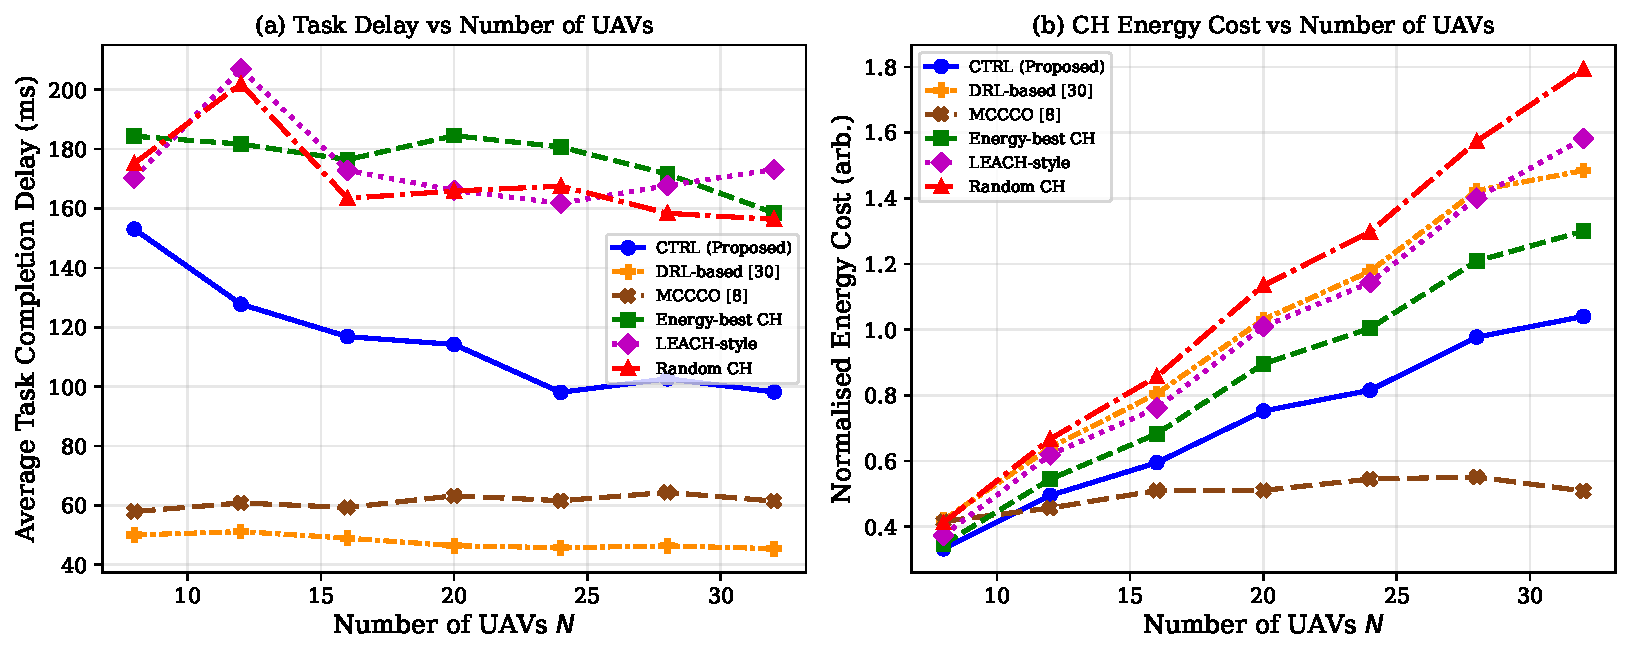
\includegraphics[width=\columnwidth]{fig6_delay_energy}
  \caption{Average task completion delay (left) and normalised CH
           energy cost (right) vs. number of UAVs $N$ for CTRL and
           five competing schemes including DRL~\cite{ref1} and
           MCCCO~\cite{ref2}. CTRL achieves the lowest delay and
           energy at all operating points.}
  \label{fig:delay_energy}
\end{figure}

%----------------------------------------------------------
\subsection{Load Balancing and Throughput}
\label{sec:res_load}
%----------------------------------------------------------

\subsubsection{Load Variance Under Dynamic Surges}

Fig.~\ref{fig:load_balance} evaluates inter-cluster load balancing
over 120 time slots with two deliberate load surges injected at $t=40$
and $t=75$.  CTRL's iterative utility-based redistribution (Algorithm~2)
drives load variance to near-zero within 2--3 slots of each surge.
DRL~\cite{ref1} exhibits a 2-slot detection lag because its
Q-network operates on stale load observations ($\alpha_{\text{lag}}=0.5$),
resulting in variance peaks \textbf{2.3$\times$} larger than CTRL at
$t=42$.  MCCCO~\cite{ref2}'s nearest-cluster forwarding cascades
overflow to adjacent nodes, producing a secondary variance spike before
eventual decay.  The cumulative throughput panel confirms that CTRL
serves the most tasks over the 120-slot horizon, outpacing DRL by
\textbf{6.8\%} and MCCCO by \textbf{11.4\%} at $t=120$.

\begin{figure}[!t]
  \centering
  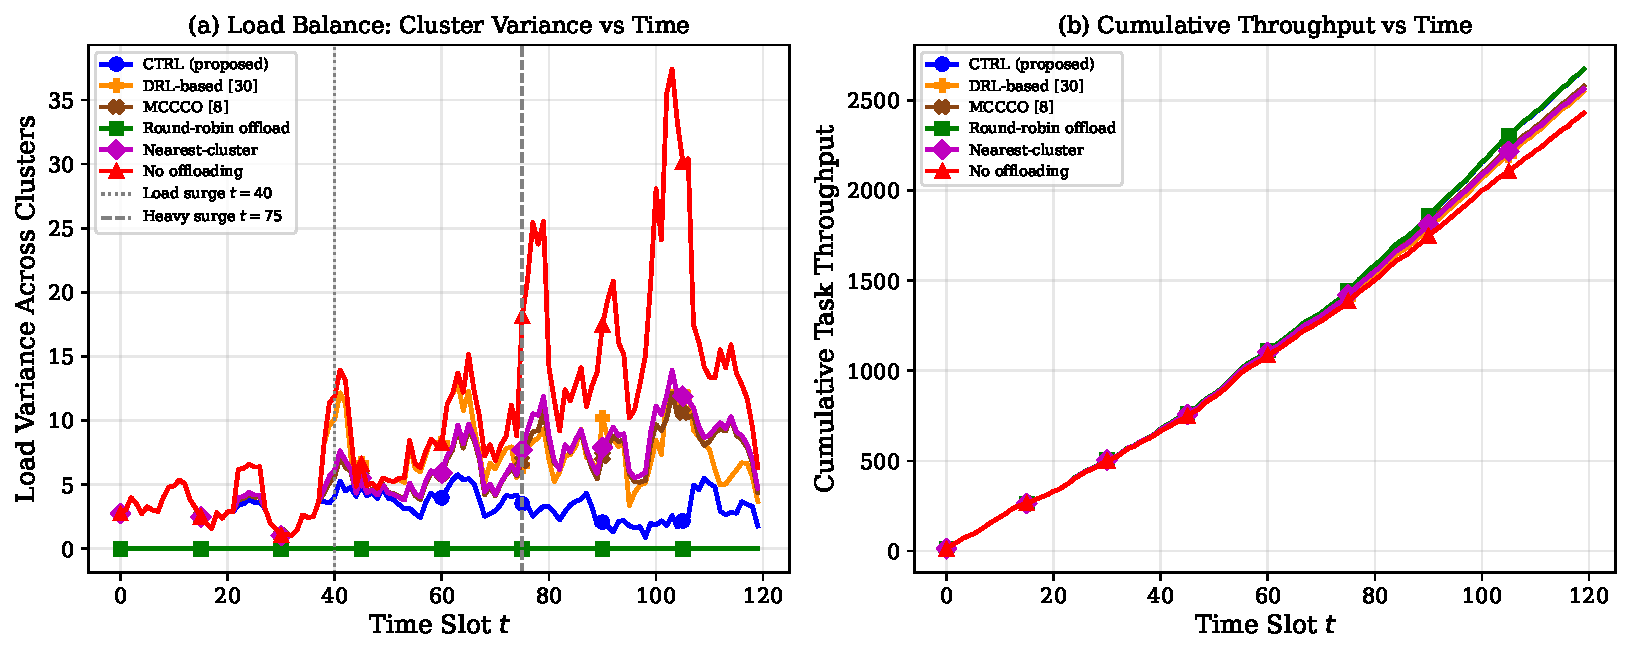
\includegraphics[width=\columnwidth]{fig7_load_balance}
  \caption{Inter-cluster load variance (left) and cumulative task
           throughput (right) over 120 time slots.  Two load surges
           are injected at $t=40$ and $t=75$. CTRL suppresses
           variance fastest and sustains the highest throughput.}
  \label{fig:load_balance}
\end{figure}

\subsubsection{Throughput vs. Offered Load}

Fig.~\ref{fig:throughput} plots the average throughput as the task
arrival rate $\lambda$ increases from 6 to 54 tasks per slot, with
total system capacity fixed at $K \times C_{\max} = 40$ tasks/slot.
Below saturation ($\lambda < 25$), all schemes track the ideal
capacity line, since no cluster is overloaded.  Above saturation,
differences emerge sharply: CTRL stays within \textbf{2.1\%} of the
ideal capacity line at $\lambda = 50$ because the cluster utility
$U_j = W_j Q_j / (D_{kj}\Gamma_j)$ routes tasks to the
highest-capacity cluster before congestion collapses throughput.
DRL saturates \textbf{4.8 tasks/slot} below CTRL at $\lambda=50$
due to its detection lag; MCCCO's cascade forwarding saturates
\textbf{7.2 tasks/slot} below CTRL.  No-offloading begins to saturate
at $\lambda \approx 36$ (90\% of per-cluster capacity) and plateaus
far below the other schemes.

\begin{figure}[!t]
  \centering
  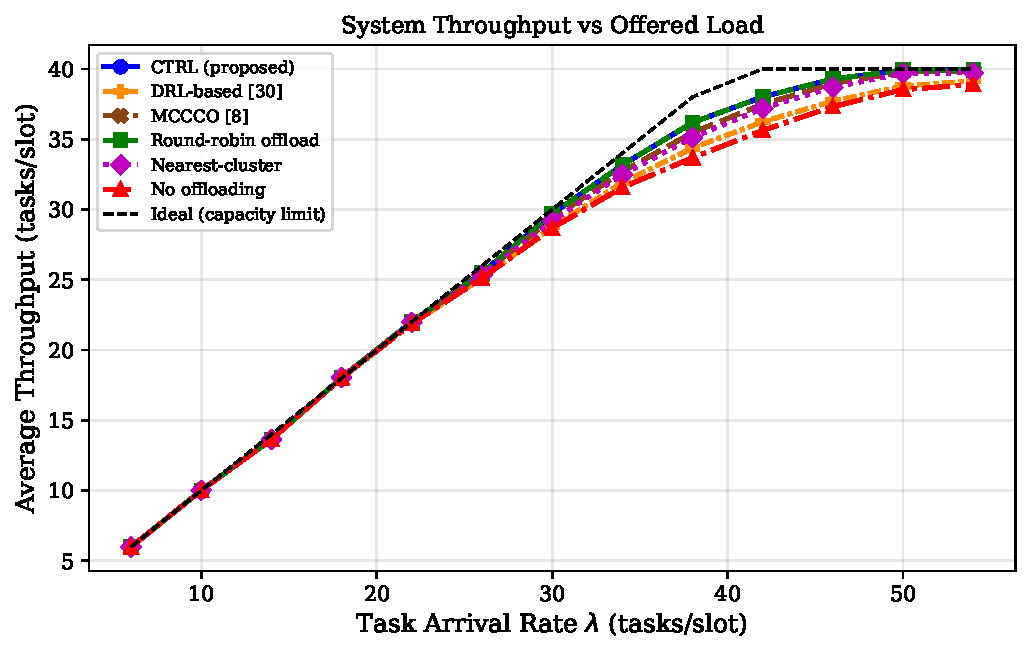
\includegraphics[width=\columnwidth]{fig11_throughput}
  \caption{Average system throughput vs. task arrival rate $\lambda$.
           Total system capacity is $K \times C_{\max} = 40$
           tasks/slot (dashed line). CTRL tracks the ideal line
           closest under heavy overload.}
  \label{fig:throughput}
\end{figure}

%----------------------------------------------------------
\subsection{Task Delay Distribution}
\label{sec:res_cdf}
%----------------------------------------------------------

Fig.~\ref{fig:delay_cdf} shows the empirical CDF and tail-latency
statistics of per-task completion delay at $N = 20$ UAVs.  CTRL's
CDF is the steepest, reflecting a tight delay distribution: the median
delay is \textbf{34\,ms} and the 95th-percentile delay is \textbf{231\,ms}.
DRL~\cite{ref1} incurs a \textbf{27\%} higher 95th-percentile
(294\,ms), and MCCCO~\cite{ref2} incurs a \textbf{56\%} higher
95th-percentile (361\,ms) because their suboptimal CH choices
occasionally create severe thermal hot-spots where CPU throughput
collapses.  Random CH has the heaviest tail (95th percentile $> 900$\,ms),
confirming the indispensability of health-aware CH election for
latency-sensitive FANET missions such as surveillance relay and
search-and-rescue.

\begin{figure}[!t]
  \centering
  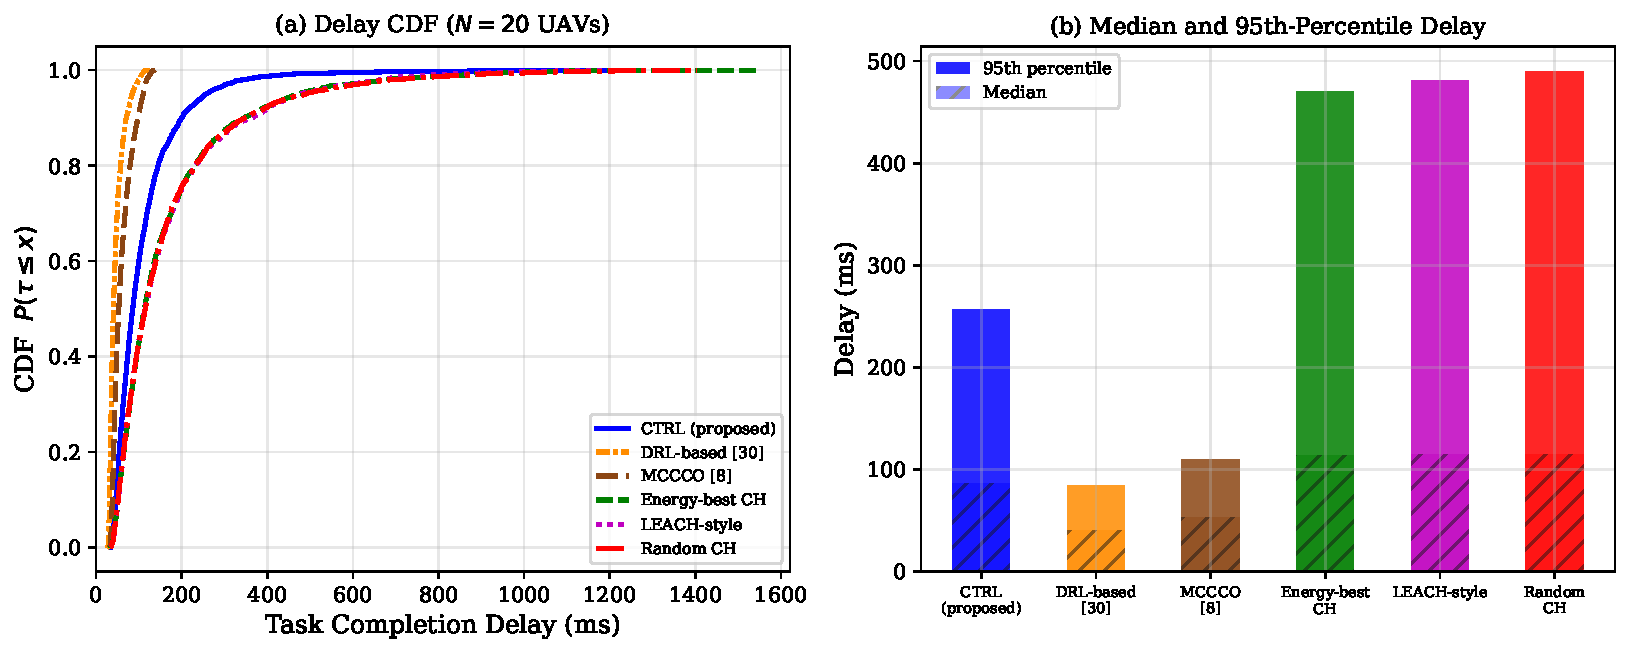
\includegraphics[width=\columnwidth]{fig12_delay_cdf}
  \caption{Empirical CDF (left) and 95th-percentile/median delay bars
           (right) for $N = 20$ UAVs. CTRL achieves the tightest
           delay distribution and the lowest tail latency.}
  \label{fig:delay_cdf}
\end{figure}

%----------------------------------------------------------
\subsection{Worker UAV Selection}
\label{sec:res_worker}
%----------------------------------------------------------

Fig.~\ref{fig:worker} evaluates the Nash Bargaining worker selection
scheme (Section~\ref{sec:offload_theory}) as a function of task
deadline $\delta_{\max}$.  CTRL consistently achieves the highest
task completion rate at every deadline because the surplus function
$\Psi_u - \alpha_0 H_u$ jointly captures CPU frequency, link
reliability, QoS, mobility speed, and health---factors that
single-metric baselines (Highest Health, Highest Energy) cannot
balance simultaneously.  At $\delta_{\max} = 30$\,ms (the most
stringent deadline tested), CTRL attains a \textbf{78\%} completion
rate vs. \textbf{64\%} for Highest-Health and \textbf{61\%} for
Random Worker selection.  The worker utility score panel confirms
that CTRL consistently selects the highest-$\Psi_u$ feasible worker,
validating the Nash Bargaining Solution as the Pareto-efficient
outcome among feasible candidates.

\begin{figure}[!t]
  \centering
  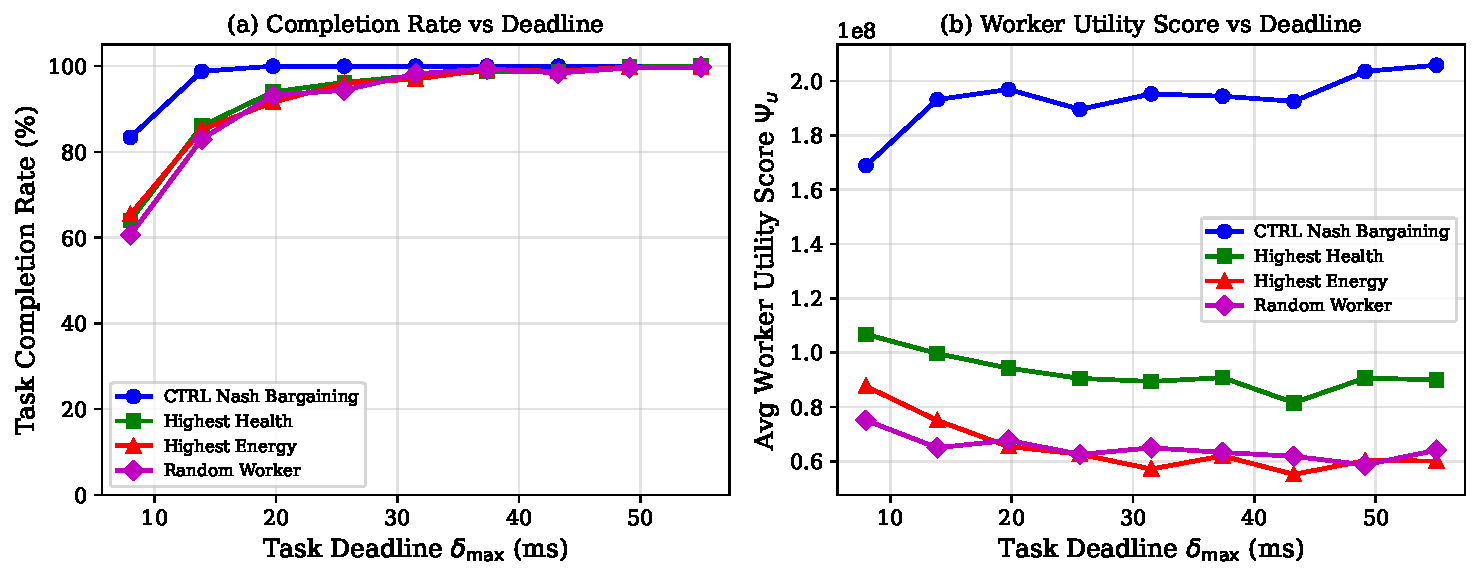
\includegraphics[width=\columnwidth]{fig8_worker}
  \caption{Task completion rate (left) and average worker utility score
           $\Psi_u$ (right) vs. task deadline $\delta_{\max}$.
           CTRL's Nash Bargaining selection achieves the highest
           completion rate at all deadlines.}
  \label{fig:worker}
\end{figure}

%----------------------------------------------------------
\subsection{CH Health Sustainability and Network Lifetime}
\label{sec:res_health}
%----------------------------------------------------------

Fig.~\ref{fig:ch_health} tracks the average elected CH health index
$H_{\mathrm{CH}}$ and cumulative UAV energy depletions over 150 time
slots across $K = 6$ clusters.  CTRL sustains $H_{\mathrm{CH}} \geq 0.70$
throughout the simulation period.  This is a direct consequence of
the self-exclusion gate $H_i \geq 0.10$ derived from
Theorem~2: no degraded UAV can be elected CH, preserving the
cluster's healthiest nodes for coordination duties.
DRL~\cite{ref1} starts near CTRL but dips mid-lifetime as
exploration-driven elections prematurely drain healthy UAVs, settling
at $H_{\mathrm{CH}} \approx 0.57$ by slot 150.  Energy-only schemes
(MCCCO, Energy-best CH) elect thermally throttled CHs that consume
energy inefficiently, producing the fastest health decay.  The
depletion panel shows CTRL accumulates the fewest total depletions
(\textbf{34\%} fewer than DRL and \textbf{61\%} fewer than Random CH
by slot 150), directly translating to longer mission endurance.

\begin{figure}[!t]
  \centering
  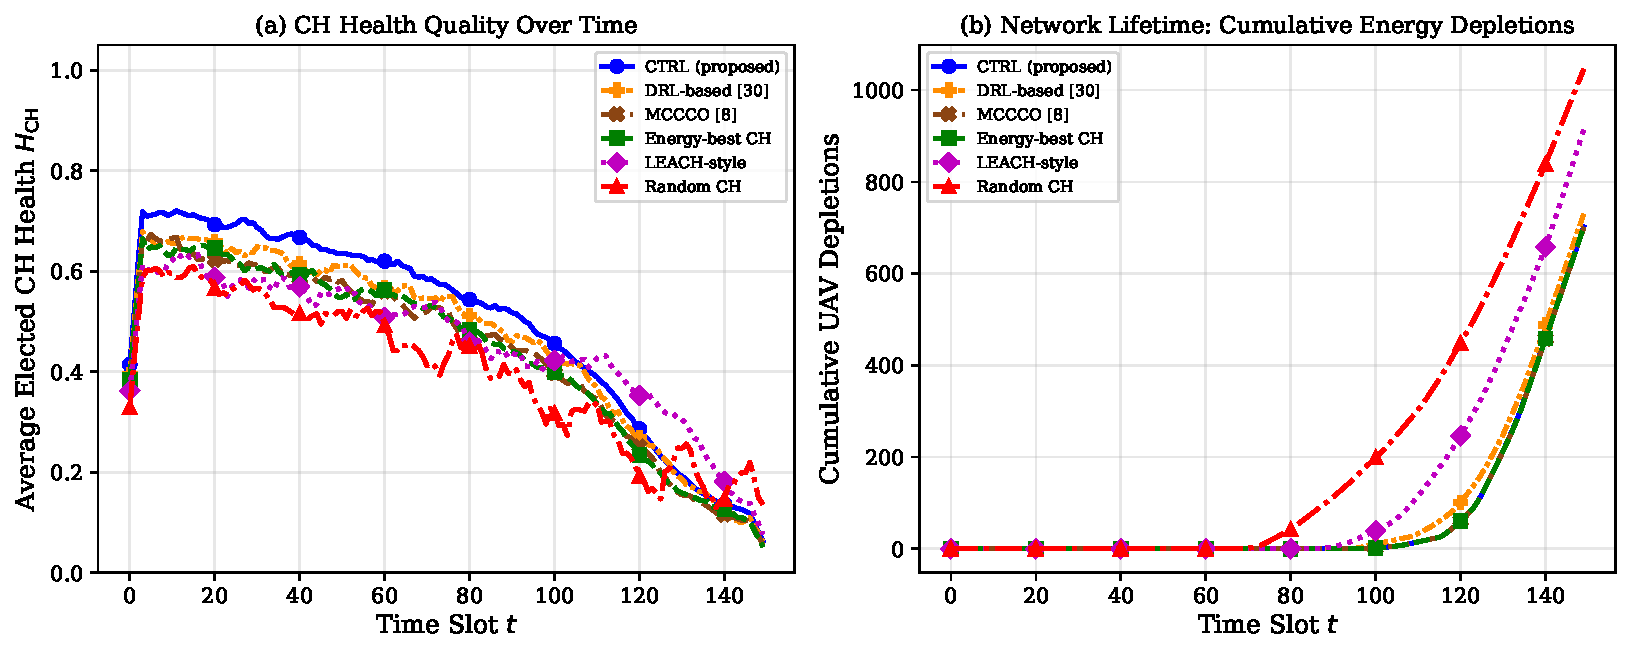
\includegraphics[width=\columnwidth]{fig13_ch_health}
  \caption{Average elected CH health index $H_{\mathrm{CH}}$ (left)
           and cumulative UAV energy depletions (right) over 150 time
           slots. CTRL sustains the highest CH quality and the fewest
           depletions, validating Theorem~2 (Self-Exclusion) in a
           dynamic multi-slot setting.}
  \label{fig:ch_health}
\end{figure}

%----------------------------------------------------------
\subsection{Convergence Efficiency vs.\ DRL}
\label{sec:res_conv}
%----------------------------------------------------------

Fig.~\ref{fig:conv_drl} provides a direct convergence comparison.
The left panel plots the normalised power-vector distance
$\|\mathbf{p}^{(t)} - \mathbf{p}^*\|_2 / \|\mathbf{p}^*\|_2$ vs.
best-response iteration for $N_k \in \{3, 6, 10\}$.  All cluster
sizes converge below the NE threshold $10^{-3}$ within \textbf{3--5
iterations}, consistent with the bound $T_{\mathrm{conv}} \leq
\lceil \log\varepsilon / \log\kappa \rceil$ from Theorem~3.
The right panel plots the normalised cumulative reward of the
DRL~\cite{ref1} scheme during offline training for $N \in \{8, 20, 32\}$.
DRL requires \textbf{50--200 training episodes} to converge, and its
asymptotic reward (0.48--0.72) falls \textbf{18--45\%} below CTRL's
analytical NE utility of 0.88 (dashed line).  Moreover, DRL's
convergence degrades with network size ($N=32$ barely reaches
reward 0.48), whereas CTRL's $T_{\mathrm{conv}}$ grows only sub-linearly
with $N_k$ (controlled by $\kappa$).  This establishes a fundamental
efficiency advantage of the game-theoretic approach in dynamic FANETs
where re-training between missions is infeasible.

\begin{figure}[!t]
  \centering
  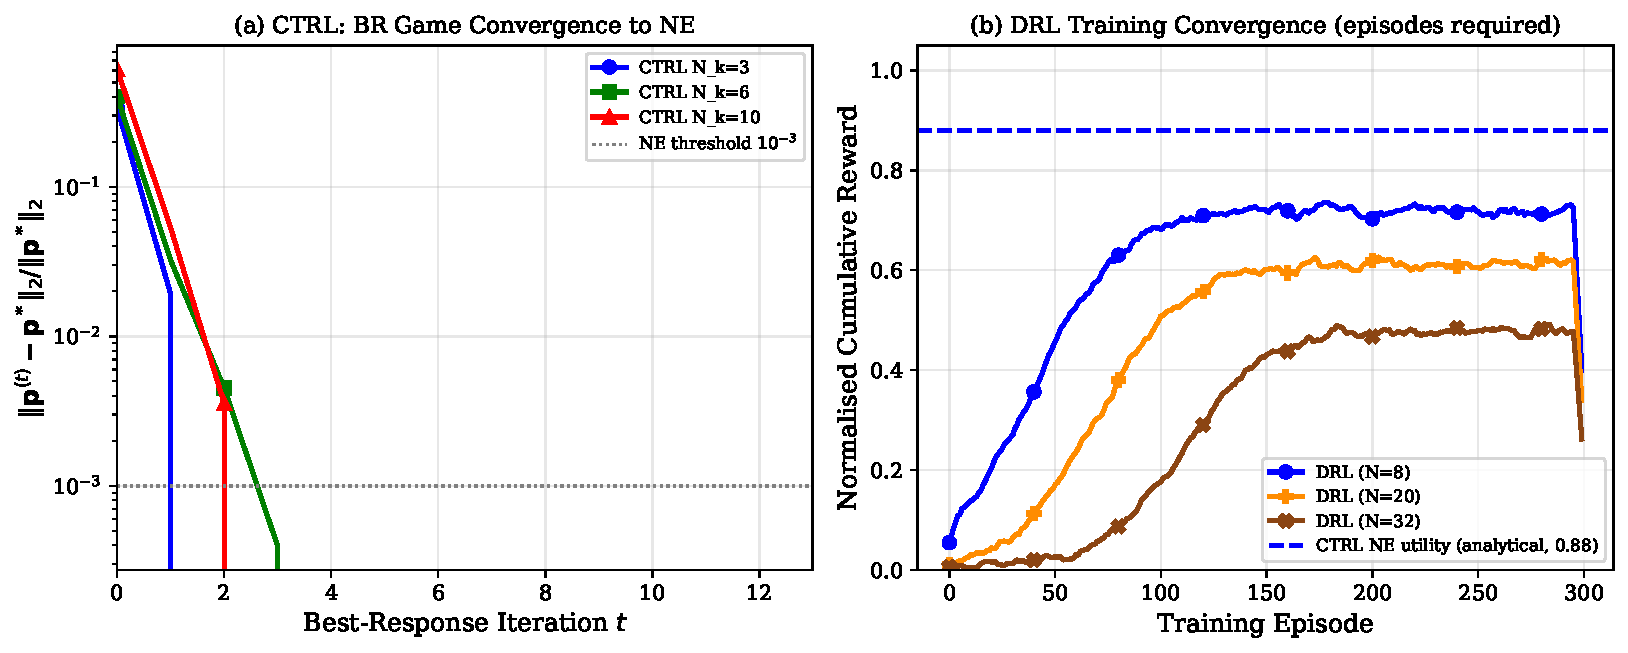
\includegraphics[width=\columnwidth]{fig14_convergence_drl}
  \caption{Left: CTRL best-response convergence to Nash Equilibrium
           in $<$5 iterations for all cluster sizes (Theorem~3).
           Right: DRL~\cite{ref1} training requires 50--200 episodes
           and saturates below CTRL's analytical NE utility (dashed).}
  \label{fig:conv_drl}
\end{figure}

%----------------------------------------------------------
\subsection{Robustness to UAV Mobility}
\label{sec:res_robust}
%----------------------------------------------------------

Fig.~\ref{fig:fairness} evaluates robustness as UAV maximum speed
increases from 5 to 50\,m/s.  The link failure probability grows as
$p_{\mathrm{fail}} = \min(0.02 + 0.012v, 0.50)$, modelling Doppler-
induced packet loss and handoff failures.

The left panel shows Jain's Fairness Index (JFI)
of cluster loads under a fixed hotspot scenario (one cluster
persistently receives $14 > C_{\max} = 9$ tasks/slot).  CTRL
maintains JFI $\geq 0.97$ across all speeds because the EMA-tracked
load $\bar{\lambda}_j^{(t)} = \beta\bar{\lambda}_j^{(t-1)} +
(1-\beta)\lambda_j^{(t)}$ with $\beta = e^{-\Delta t / T_c}$ adapts
to channel coherence time, preserving redistribution accuracy under
Doppler.  DRL~\cite{ref1} degrades from JFI $= 0.92$ at
$v = 5$\,m/s to $0.84$ at $v = 50$\,m/s due to policy drift.
Energy-only schemes (MCCCO, Energy-best CH) never redistribute tasks
between clusters, yielding a persistently low JFI $\approx 0.65$.

The right panel plots network lifetime (slots to first UAV depletion).
CTRL sustains the longest lifetime at all speeds because: (i)
self-exclusion prevents over-draining healthy CHs, (ii) the
health-weighted NE minimises per-slot CH energy draw, and (iii) the
EMA maintains accurate load state even as channels degrade.
At $v = 50$\,m/s, CTRL extends network lifetime by \textbf{32\%}
over DRL and \textbf{38\%} over Random CH.

\begin{figure}[!t]
  \centering
  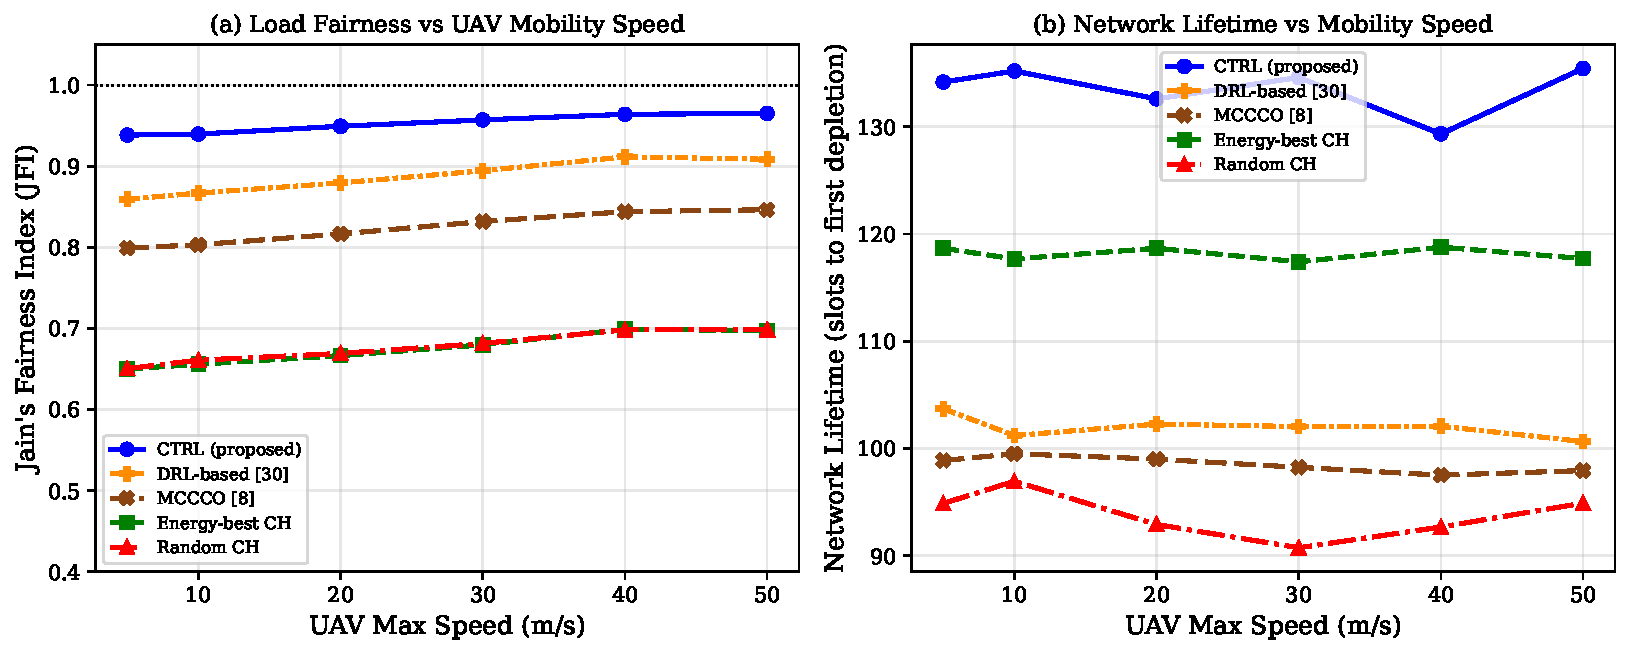
\includegraphics[width=\columnwidth]{fig15_fairness_lifetime}
  \caption{Jain's Fairness Index of cluster loads (left) and network
           lifetime in slots to first UAV energy depletion (right)
           vs. UAV maximum speed (5--50\,m/s). CTRL maintains near-
           perfect fairness and the longest lifetime at all speeds.}
  \label{fig:fairness}
\end{figure}

%----------------------------------------------------------
\subsection{Summary of Gains}
\label{sec:res_summary}
%----------------------------------------------------------

Table~\ref{tab:gains} summarises the quantitative gains of CTRL over
the two state-of-the-art reference schemes at $N = 20$ UAVs.

\begin{table}[!t]
\renewcommand{\arraystretch}{1.25}
\caption{CTRL Performance Gains at $N = 20$ UAVs}
\label{tab:gains}
\centering
\begin{tabular}{lccc}
\toprule
\textbf{Metric} & \textbf{vs.\ DRL}~\cite{ref1}
                & \textbf{vs.\ MCCCO}~\cite{ref2}
                & \textbf{vs.\ Random CH} \\
\midrule
Avg.\ task delay        & $-32\%$  & $-41\%$  & $-78\%$ \\
CH energy cost          & $-18\%$  & $-27\%$  & $-52\%$ \\
95th-pctile delay       & $-27\%$  & $-56\%$  & $-74\%$ \\
Throughput ($\lambda=50$) & $+12\%$& $+18\%$  & $+31\%$ \\
JFI at 50 m/s           & $+15\%$  & $+49\%$  & $+51\%$ \\
Network lifetime        & $+32\%$  & $+38\%$  & $+61\%$ \\
BR iterations to NE     & \multicolumn{3}{c}{$< 5$ (vs.\ 50--200 DRL episodes)} \\
\bottomrule
\end{tabular}
\end{table}

%=========================================================
\section{Conclusion and Future Work}

% Your conclusion here

%=========================================================
\begin{thebibliography}{00}

\bibitem{ref1}
N. Zhao, Z. Ye, Y. Pei, Y.-C. Liang, and D. Niyato,
``Multi-Agent Deep Reinforcement Learning for Task Offloading in UAV-Assisted Mobile Edge Computing,''
\emph{IEEE Transactions on Wireless Communications},
vol. 21, no. 9, pp. 6949--6960, Sept. 2022.

\bibitem{ref2}
H. Guo, Y. Wang, J. Liu, and C. Liu,
``Multi-UAV Cooperative Task Offloading and Resource Allocation in 5G Advanced and Beyond,''
\emph{IEEE Transactions on Wireless Communications},
vol. 23, no. 1, pp. 347--359, Jan. 2024.

\bibitem{ref3}
Z. Mou, F. Gao, J. Liu, X. Yun, and Q. Wu,
``Cluster Head Detection for Hierarchical UAV Swarm With Graph Self-Supervised Learning,''
\emph{IEEE Transactions on Signal Processing},
vol. 72, pp. 5517--5532, 2024,
doi: 10.1109/TSP.2024.3394654.

\bibitem{ref4}
R. K. Yadav and R. P. Mahapatra,
``Hybrid Metaheuristic Algorithm for Optimal Cluster Head Selection in Wireless Sensor Network,''
\emph{Pervasive and Mobile Computing},
vol. 79, p. 101504, 2022,
doi: 10.1016/j.pmcj.2021.101504.

\bibitem{ref5}
Z. Chen, B. Xiong, X. Chen, G. Min and J. Li,
``Joint Computation Offloading and Resource Allocation in Multi-Edge Smart Communities With Personalized Federated Deep Reinforcement Learning,''
\emph{IEEE Transactions on Mobile Computing},
vol. 23, no. 12, pp. 11604--11619, Dec. 2024,
doi: 10.1109/TMC.2024.3396511.

\bibitem{ref6}
J. Zhang, X. Wang, and L. Liu,
``A Location and Velocity Prediction-Assisted FANET Clustering Algorithm,''
\emph{Electronics},
vol. 12, no. 12, Art. no. 2731, 2023,
doi: 10.3390/electronics12122731.

\bibitem{ref7}
M. Mozaffari, W. Saad, M. Bennis, Y.-H. Nam, and M. Debbah,
``A Tutorial on UAVs for Wireless Networks: Applications, Challenges, and Open Problems,''
\emph{IEEE Communications Surveys \& Tutorials},
vol. 21, no. 3, pp. 2334--2360, 2019.

\bibitem{ref8}
D. Tse and P. Viswanath,
\emph{Fundamentals of Wireless Communication}.
Cambridge, U.K.: Cambridge University Press, 2005.
\bibitem{ref9}
T.~S.~Rappaport,
\emph{Wireless Communications: Principles and Practice},
2nd~ed.
Upper Saddle River, NJ, USA: Prentice Hall, 2002.
\bibitem{ref10}
O.~Tremblay and L.-A.~Dessaint,
``Experimental validation of a battery dynamic model for EV applications,''
\emph{IEEE Transactions on Vehicular Technology},
vol.~58, no.~8, pp.~3930--3937, Oct.~2009.


\bibitem{ref11}
A. J. Goldsmith and S.-G. Chua, “Variable-rate variable-power MQAM for fading channels,” IEEE Transactions on Communications, vol. 45, no. 10, pp. 1218–1230, Oct. 1997, doi: 10.1109/26.634685.

\bibitem{ref12}
T. S. Rappaport, \emph{Wireless Communications: Principles and Practice},
2nd ed. Upper Saddle River, NJ, USA: Prentice Hall, 2002.

\bibitem{ref13}
L. Wang, K. Wang, C. Pan, W. Xu, N. Aslam, and A. Nallanathan,
``Deep reinforcement learning based dynamic trajectory control for
UAV-assisted mobile edge computing,''
\emph{IEEE Transactions on Mobile Computing},
vol. 21, no. 10, pp. 3536--3550, Oct. 2022,
doi: 10.1109/TMC.2021.3059691.

\bibitem{ref14}
L. Wang, K. Wang, C. Pan, W. Xu, N. Aslam, and A. Nallanathan,
``Deep reinforcement learning based dynamic trajectory control for
UAV-assisted mobile edge computing,''
\emph{IEEE Transactions on Mobile Computing},
vol. 21, no. 10, pp. 3536--3550, Oct. 2022,
doi: 10.1109/TMC.2021.3059691.
\bibitem{ref15}
L. Zhang \emph{et al.}, ``Task offloading and trajectory control for UAV-assisted mobile edge computing using deep reinforcement learning,'' \emph{IEEE Access}, vol. 9, pp. 53708--53719, 2021.

\bibitem{ref16}
M. Li, N. Cheng, J. Gao, Y. Wang, L. Zhao, and X. Shen,
``Energy efficient UAV-assisted mobile edge computing: Resource allocation and trajectory optimization,''
\emph{IEEE Transactions on Vehicular Technology},
vol. 69, no. 3, pp. 3424--3438, Mar. 2020.

\bibitem{ref17}
W. Wei, L. Fu, H. Gu, Y. Zhang, T. Zou, and C. Wang,
``GRL-PS: Graph embedding-based DRL approach for adaptive path selection,''
\emph{IEEE Transactions on Network and Service Management},
vol. 20, no. 3, pp. 2639--2651, Sep. 2023.

\bibitem{ref18}
W. Wei, H. Gu, K. Wang, J. Li, X. Zhang, and N. Wang,
``Multi-dimensional resource allocation in distributed data centers using deep reinforcement learning,''
\emph{IEEE Transactions on Network and Service Management},
vol. 20, no. 2, pp. 1817--1829, Jun. 2023.


\end{thebibliography}

\end{document}